\chapter{STATISTICALLY EFFICIENT ACTOR--CRITIC METHODS}
\label{ch:actor-critic}

\aigen{\emph{This chapter is based on joint work with Wei Fan and Yuting Wei \citep{tan2025actor}: Kevin Tan, Wei Fan, and Yuting Wei, ``Actor-Critics Can Achieve Optimal Sample Efficiency, in Proceedings of the 42nd International Conference on Machine Learning (ICML), PMLR 267, 2025. The dissertation author carried out the problem formulation, algorithm design, experiments, and writing, with the theoretical analysis and proofs developed jointly with Wei Fan.}}

\section{Introduction}
% \section{Background and motivation}
% Problems with Zhou:
% \begin{enumerate}
%     \item Requirement of Monte Carlo rollouts and sampling on-policy at each policy evaluation iteration. Why can't you just minimize error under some buffer? 
%     \begin{itemize}
%         \item They need this to get the NPG-style online guarantee. Otherwise they would need full offline RL concentrability guarantees. That could be weakened to partial concentrability, but requires exploration. Need optimistic policy gradient/actor critic, e.g. OPPO. 
%         \item This means that they really sample $O(T^2\sqrt{T})$ online samples during the $\sqrt{T}$ rounds of regret-minimization
%     \end{itemize}
%     \item NPG coefficient is on the order of the square of the single-policy concentrability when the behavior dataset is generated by some policy. Need optimistic exploration, e.g. optimistic critics or optimistic PPO (https://arxiv.org/pdf/1912.05830), to get rid of this. Do regression on the neural tangent kernel features in order to handle general function approximation while using linear MDP-style bonuses. 
%     \begin{itemize}
%         \item NPG coefficient can be relaxed to a variant of squared Bellman error concentrability where we take a maximum over all behavior policies in the denominator, and have the optimal policy in the numerator. 
%     \end{itemize}
%     \item We wish to weaken concentrability over the entire state space to partial concentrability. Even if single-policy concentrability, the all-policy partial concentrability can still be bounded when SPC is unbounded. Consider the following two approaches:
%     \begin{itemize}
%         \item We use the MWU update as in the HAC algorithm for the policy, and use an optimistic critic as in the GOLF algorithm. This should realize some $\inf_{\gX_{\off}, \gX_{\on}}\sqrt{\log(|\gF|)c_{\off}(\gF, \gX_{\off})H^4T^2/N_{\off}} + \sqrt{\log(|\gF|)c_{\on}(\gF, \gX_{\on})H^4T}+ \sqrt{\log(|\gF|)H^4T}$, where the last term is modulo some potential change in measure from the optimal policy occupancy measure to the on-policy occupancy measure. That is, we want to bound
%         $$\sum_{h,t} \E_{s \sim d_h^{(t)}}[f_h^{(t)}(s,a^*) - f_h^{(t)}(s,\pi_h^{(t)}(s))],$$
%         which they require the $C_{\text{npg}, \pi^e}$ coefficient to get a change of measure to. This can be bounded by the policy improvement step arguments in the OPPG paper. 
%     \end{itemize}
%     \item Use neuraltangents or JAX to get NTK regression done for the critic to effectively perform optimism, and have the actor parametrized by a standard neural network. 
% \end{enumerate}


Actor-critic algorithms have emerged as a foundational approach in reinforcement learning (RL), mitigating the deficiencies of both policy-based and value-based approaches \citep{sutton1998, mnih2016asynchronousmethodsdeepreinforcement, haarnoja2018soft}. 
These methods combine two components: an actor, which directly learns and improves the policy, and a critic, which evaluates the policy's quality. 
Given their popularity, significant recent progress has been made in understanding their theoretical underpinnings and statistical efficiency, especially in the presence of function approximation \citep{cai2020provably, zhong2023theoretical, sherman2023rate, liu2023optimistic} -- which is required in real-world applications with prohibitively large state and action spaces.

% \textbf{Optimization perspectives.} 
However, much existing work \citep{abbasi2019politex, neu2017unified, liu2023neuralproximaltrustregionpolicy, bhandari2024global, agarwal2021theory, cen2022fast, gaur2024closing} on the convergence of actor-critic methods requires assumptions on the reachability of the state-action space or on the coverage of the sampled data. \citet{liu2023optimistic} remark that this implies that the state-space is either well-explored or easy to explore. This allows the agent to bypass the need to actively explore the state-action space, making learning significantly easier.\footnote{When coverage/reachability assumptions are made, the linear convergence of policy-based methods \citep{lan2022policymirrordescentreinforcement, xiao2022convergence, yuan2023linear, chen2022offpolicylinearpolicy} and the gradient domination lemma \citep{kumar2024improvedsamplecomplexityglobal, mei2022globalconvergenceratessoftmax} enable the natural actor-critic algorithm to learn an $\epsilon$-optimal policy within $1/\epsilon^2$ samples if one can access the exact NPG update, although vanilla policy gradient methods can take (super) exponential time to converge \citep{li2021softmax}.} Therefore, these approaches analyze actor-critic methods from an optimization perspective and do not address the problem of exploration \citep{efroni2020optimisticpolicyoptimizationbandit} -- a salient problem that we seek to tackle, hence the need for strategic exploration. 

% \textbf{Strategic exploration.} 
Without reachability assumptions, policy gradient methods struggle due to a lack of strategic exploration.\footnote{To illustrate, this was not solved until \citet{agarwal2020pcpgpolicycoverdirected}, who required $1/\epsilon^{11}$ samples to do so in linear MDPs.} A recent line of work utilizes optimism to address this. \citet{efroni2020optimisticpolicyoptimizationbandit, wu2022nearlyoptimalpolicyoptimization} and \citet{cai2020provably} achieve $\sqrt{T}$ regret within the settings of tabular and linear mixture MDPs respectively, with \citet{wu2022nearlyoptimalpolicyoptimization} attaining the minimax-optimal rate.  
Still, \citet{zhong2023theoretical, liu2023optimistic} remark that these analyses do not generalize to more general MDPs due to the need to cover an exponentially growing policy class. Optimism is not the only way to solve this issue. For instance, \citet{huang2024sublinearregretclasscontinuoustime} utilize Gaussian perturbations to perform exploration in the linear-quadratic control problem. However, naive, direction-unaware perturbation-based exploration comes with a cost, achieving only $T^{3/4}$ regret in this case.

% \textbf{Function approximation.} 
Within linear MDPs, \citet{sherman2023rate} and \citet{cassel2024warm} have very recently been able to obtain the optimal rate of $\sqrt{T}$ regret or $1/\epsilon^2$ sample complexity. They do so via methodological advancements (specific to linear MDPs) that let them overcome the growing policy class issue.
However, the problem is unresolved with general function approximation -- the best known algorithm from \citet{liu2023optimistic} requires at least $1/\epsilon^3$ samples, increasing to $1/\epsilon^4$ when the policy class grows exponentially.


%For example, GOLF, which is designed to learn near-optimal policies in problems with low Bellman Eluder dimension (a concept we define later), still exhibits a sample complexity that is polynomial in all relevant parameters, albeit independent of the size of state-action space.

\paragraph{An open problem.} \textit{No actor-critic algorithm with general function approximation is currently known to achieve $1/\epsilon^2$ sample complexity or $\sqrt{T}$ regret} in this more challenging setting where strategic exploration is necessary. \citet{zhong2023theoretical} and \citet{liu2023optimistic} remark that  a way forward to achieve the desired $1/\epsilon^2$ sample complexity remains unclear, and raise the open problem:

\begin{center}
    \textit{Can actor-critic or policy optimization algorithms achieve $1/\epsilon^2$ sample complexity or $\sqrt{T}$ regret with general function approximation and when strategic exploration is necessary?}
\end{center}



\begin{table*}[t!]
    \centering
    \scalebox{0.69}{
    \begin{tabular}{c|c|c|c}
    \toprule
        Algorithm & Sample Complexity & Regret & Remarks \tabularnewline
        \toprule
        
        \citet{agarwal2020pcpgpolicycoverdirected} &  $ d^3H^{15}\log|\gA|/\epsilon^{11}$ &
        None &
        \tabularnewline
        \citet{zanette2021cautiously} & $H^4\log|\gA|/\epsilon^2 + d^3H^{13}\log|\gA|/\epsilon^3$ &
        $\sqrt{H^4\log|\gA|\log|\gA|T} + \sqrt{d^3H^{13}T}$& \centering \vline
        \tabularnewline
        \citet{zhong2023theoretical} & $d^3H^8\log|\gA|/\epsilon^4 + d^5H^4/\epsilon^2$ &
        $\sqrt{d^3H^8\log|\gA|T} + \sqrt{d^5H^4T}$&Linear MDPs only
        \tabularnewline
        \citet{sherman2023rate}& $d^4H^7\log|\gA|/\epsilon^2$ & $\sqrt{d^4H^7\log|\gA|T}$ & \centering \vline
        \tabularnewline
        \citet{cassel2024warm} & 
        $dH^5\log|\gA|/\epsilon^2 + d^3H^4/\epsilon^2$
        & $\sqrt{dH^5\log|\gA|T} + \sqrt{d^3H^4T}$
        & 
        \tabularnewline
        \toprule
        \citet{zhou2023offline} & $(\log|\gA|+C_{\text{npg}}^3\wedge C_{\off}^6)\log|\gF|H^{14}/\epsilon^6$& Linear & Requires offline data
        \tabularnewline
        \citet{liu2023optimistic} & $d\log|\gA|\log|\gF|H^6/\epsilon^3$& None & ``Good'' case only, $1/\epsilon^4$ generally 
        
        \tabularnewline
        \aigen{Algorithm~\ref{alg:DOUHUA} (Sec.~\ref{sec:douhua-easy})} & $\tcbhighmath[colframe=ballblue]{H^4\log|\gA|/{\epsilon^2} + dH^4\log|\gF|/\epsilon^2}$ & $\tcbhighmath[colframe=ballblue]{\sqrt{H^4\log|\gA|T} + \sqrt{dH^4\log|\gF|T}}$ & ``Good'' case only, vacuous generally
        
        \tabularnewline
        \aigen{Algorithm~\ref{alg:NORA} (Sec.~\ref{sec:nora-hard})} & $\tcbhighmath[colframe=red]{dH^5\log|\gA|/{\epsilon^2} + dH^4\log|\gF|/{\epsilon^2}}$ & $\tcbhighmath[colframe=red]{\sqrt{dH^5\log|\gA|T} + \sqrt{dH^4\log|\gF|T}}$ & 
        Holds generally
        \tabularnewline
        \bottomrule
    \end{tabular}
    }
    \caption[Comparison of sample complexity and regret bounds for online actor--critic methods]{Comparison of our work to existing literature. Algorithm~\ref{alg:NORA} achieves the best known bound for actor-critic methods with general function approximation, and resolves an open problem on whether $\sqrt{T}$ regret or $1/\epsilon^2$ sample complexity is achievable in this scenario.}
    \label{tab:bounds-ac}
\end{table*}



\section{Contributions of Part I}
We resolve this open problem in the affirmative. As a warm-up, we first consider an easy case -- where the complexity of the class of policies considered by the policy optimization procedure does not increase exponentially with the number of (critic) updates.\footnote{It was previously considered in \citet{zhong2023theoretical} that the log-covering number of the policy class increases in the number of actor and critic updates.  
We sharpen this bound to the number of critic updates in Lemma \ref{lem:b2-covering-number-policy}, which may be of independent interest.} Then, a simple modification to the GOLF algorithm of \citet{jin2021bellmaneluder} (Algorithm~\ref{alg:DOUHUA} in Section~\ref{sec:douhua-easy}) allows one to achieve a regret of $\sqrt{H^4\log|\gA|T} + \sqrt{dH^4 \log|\gF| \;T}$,
in line with the results of \citet{efroni2020optimisticpolicyoptimizationbandit, cai2020provably} for tabular and linear mixture MDPs respectively.


However, this is not the case in many practical scenarios -- for example, where one uses linear models, decision trees, neural networks, or even random forests for the critic. In this much harder setting, Algorithm~\ref{alg:DOUHUA} cannot achieve sublinear regret. We address this by introducing a rare-switching optimistic actor-critic with uniform policy resets (Algorithm~\ref{alg:NORA} in Section~\ref{sec:nora-hard}), which leverages three crucial ingredients: (1) optimism, (2) off-policy learning, and (3) rare-switching critic updates that target $Q^*$ and accompanying policy resets. Algorithm~\ref{alg:NORA} achieves $\sqrt{d H^4 \log|\gF| T} + \sqrt{dH^5 \log|\mathcal{A}|T}$ regret, requiring only a factor of $dH\log T$ more samples than Algorithm~\ref{alg:DOUHUA} even in the best case for the latter.




%The critic targets $Q^*$ and not $Q^\pi$ in order to ensure optimism with respect to every potential policy. As the critic targets $Q^*$, there is no issue of computing $\log |(\gT^\Pi)^T \gF|$ as the Bellman operator under the greedy policy is a contraction. However, a technical issue then arises, introducing the need to perform policy resets at every critic update to alleviate this. The use of rare-switching critic updates as in \citep{he2023nearly, zhao2023nearlyoptimallowswitchingalgorithm, xiong2023generalframeworksequentialdecisionmaking} then allows us to control the additional error that arises. 

%and accompanying resets can be seen theoretically as bypassing the issue of covering a prohibitively large policy space raised by \citet{zhong2023theoretical, liu2023optimistic}, and practically as choosing batch sizes adaptively to balance the frequency and noisiness of gradient updates.  and to alleviate a technical issue with regard to the rare-switching critic updates that elaborate on later. 

\section{Extensions to hybrid RL}

\citet{zhou2023offline} use both offline and online data to bypass the need to perform strategic exploration in policy optimization. This corresponds to the setting of hybrid RL \citep{nakamoto2023calql, amortila2024harnessing, ren2024hybrid, wagenmaker2023leveraging}, where \citet{song2023hybrid} show that using both offline and online data allows one to achieve $\sqrt{T}$ regret without optimism. However, the claimed $\sqrt{T}$ regret bound in \citet{zhou2023offline} requires on-policy sampling of $O(T)$ samples per timestep that does not contribute to the regret, leading to a sample complexity of $1/\epsilon^6$. Their algorithm cannot achieve sublinear regret in the more common setup where each sample contributes to the regret. Furthermore, they require bounded occupancy measure ratios of the optimal policy to \textit{any} policy.

We demonstrate that these issues can be mitigated. Specifically, we extend our optimistic algorithm to leverage both offline and online data, and show that actor-critic methods can benefit from hybrid data and achieve the provable gains in sample efficiency as observed in \cite{li2023reward, tan2024natural, tan2024hybrid}. We also provide a non-optimistic provably efficient actor-critic
algorithm that only additionally requires $N_{\off} \geq c_{\off}^*(\gF,\Pi)dH^4/\epsilon^2$ offline samples (with bounded single-policy concentrability) in exchange for omitting optimism. This, along with the result in Theorem \ref{thm:hybrid-nora-regret_bound}, shows that hybrid RL therefore allows for sample efficiency gains with optimistic algorithms and computational efficiency gains with non-optimistic algorithms. 


% \textbf{Technical challenges.} There remains the technical issue raised in \citep{zhong2023theoretical, liu2023optimistic} on the covering of a prohibitively large policy space. This arises because one needs to bound the covering number of the value function class. 
% \citet{zhong2023theoretical} assert that one either incurs a $|\gA|$ dependence in the log-covering number of the policy class, or accepts that the log-covering number of the resulting value function class induced by Bellman backups with respect to stochastic policies grows linearly in the number of updates. 

% This is not the only setting where this is an issue -- \citet{he2023nearly} find that this arises when needing to ensure the monotonicity of their value function estimates. Our first technical contribution is in adapting the rare-switching framework of \citet{xiong2023generalframeworksequentialdecisionmaking} to the policy optimization setting. This allows us to reduce the number of critic updates, and thereby the growth of the log-covering number, from $O(\sqrt{T})$ in \citep{zhong2023theoretical, liu2023optimistic} to $O(dH\log T)$. Crucially, the result from \citet{zhong2023theoretical} that the log-covering number of the value function class grows in the number of actor-critic updates is insufficient to obtain our desired bound. To achieve our result, we needed to show that the log-covering number only increases in the number of \textit{critic} updates, not policy updates. 

% This allows us to bound the $\rho$-log-covering number of the value function class by $O(\min\{|\gA|+\log \gN_{\gF}(\rho), dH\log T\log \gN_{\gF}(\rho/H)\}))$, which is the tool that ultimately allows us to achieve $\sqrt{T}$ regret and $1/\epsilon^2$ sample complexity. In contrast, the $O(\sqrt{T})$ updates that \citep{zhong2023theoretical, liu2023optimistic} require lead to a regret of $T^{3/4}$ for the former and a sample complexity of $1/\epsilon^3$ for the latter. 

%Our second technical contribution is in developing methodology for implementing optimism when the actor is parametrized by a neural network. Although this was first proposed for contextual bandits by \citet{zhou2020neuralcontextualbanditsucbbased}, implementing optimism through the use of neural tangent prediction intervals has not been done in RL. To do so, we leverage the equivalence between the natural policy gradient update for a log-linear policy class parametrized with neural tangent kernel features and natural policy gradient with a neural network actor \citep{zhou2023offline}. We provide an end-to-end regret bound for this procedure that depends on the effective dimension as in \citet{zhou2020neuralcontextualbanditsucbbased} and not the norm of parameters in the neural network as in \citet{zhou2023offline}.\footnote{Although the regret bound as presented in \citet{zhou2023offline} is independent of the number of parameters, there is a linear dependence in the number of parameters that shows up in the number of on-policy and offline samples required for policy evaluation. This consequently affects the sample complexity by this amount.} We remark that the former can be significantly smaller than the latter, and achieving this dependence in the context of RL is nontrivial.

\paragraph{Notation.} We write $\gN_A(\rho)$ for the $\rho$-covering number over a set $A$, and in a small abuse of notation use $\gN_{A,B}(\rho)$ to denote the $\rho$-covering number over the set $A \cup B$. We use standard big-O and little-O notation within this chapter. $O(g(n))$ denotes the set of functions $f(n)$ such that there exist positive constants $C$ and $n_0$ such that $0 \leq f(n) \leq C\cdot g(n)$ for all $n \geq n_0$. When we say a function is $O(g(n))$, we say that it grows no faster than $g(n)$ asymptotically.
$o(g(n))$ denotes the same, except that the inequality $0 \leq f(n) < C\cdot g(n)$ is strict, and so grows strictly slower than $g(n)$ asymptotically. $\Omega(g(n))$ involves the inequality $0 \leq C\cdot g(n) \leq f(n)$, and so denotes the set of functions $f(n)$ that grow at least as fast as $g(n)$. Finally, $\Theta(g(n))$ denotes the set of functions that are both $O(g(n))$ and $\Omega(g(n))$.


\section{Problem setting}
\label{sec:ch04-part1-prelim}




\paragraph{Markov decision processes.}
Part~I of this chapter focuses on finite horizon, episodic MDPs, represented by a tuple
$$\mathcal{M} = (\mathcal{S},\mathcal{A}, H,\{\prob_h\}_{h=1}^{H} ,\{r_h\}_{h=1}^{H}),$$
where $\mathcal{S}$ is the state space, $\mathcal{A}$ is the action space, $H$ is the horizon, $r_h: \mathcal{S}\times\mathcal{A}\to[0,1]$ is the reward function at step $h$ and $\prob_h: \mathcal{S}\times\mathcal{A}\to\Delta(\mathcal{S})$ is the transition kernel for step $h$. A policy $\{\pi_h\}_{h=1}^{H}$ is a set of $H$ functions, where each $\pi_h:\mathcal{S}\to\Delta(\mathcal{A})$ maps from a state on step $h$ to a probability distribution on actions. Write $\Pi$ for the class of all policies, and $\pi(s)$ as shorthand for the random variable $a \sim \pi(\cdot | s)$. Given a policy $\{\pi_h\}_{h=1}^{H}$ and reward function $\{r_h\}_{h=1}^{H}$, the state value function is defined as 
\begin{align}
    V_h^{\pi}(s) = \mathbb{E}\bigg[\sum_{h'=h}^{H}r_{h'}(s_{h'},a_{h'})|s_h = s\bigg],
\end{align}
where the expectation is taken over the randomness of $a_{h'}\sim \pi_{h'}(s_{h'})$ and $s_{h'+1}\sim \prob_h(\cdot|s_{h'},a_{h'})$ for any $h'\geq h$. The action value, or Q function is defined as
\begin{align}
Q_h^{\pi}(s,a) = \mathbb{E}\bigg[\sum_{h'=h}^{H}r_{h'}(s_{h'},a_{h'})|s_h = s,a_h=a\bigg],
\end{align}
where the expectation is taken over the similar randomness of action and state transition, with the only difference that the action randomness is only random as $h'\geq h+1$.

Without loss of generality, write $s_1$ for the initial state. The optimal policy is $\pi^{\star} = \mathrm{argmax}_{\pi\in\Pi} V_1^{\pi}(s_1)$. Correspondingly, we denote $V^{\star} = V^{\pi^{\star}}$ and $Q^{\star} = Q^{\pi^{\star}}$ as the optimal value and Q-functions. The Bellman operator with respect to the greedy policy and any policy $\pi$ is given by
\begin{subequations}
\begin{align}
    \mathcal{T}_{h}Q_{h+1}(s,a) &= r_h(s,a) + \mathbb{E}_{s'\sim P_h}\Big[\max_{a'\in\mathcal{A}}Q_{h+1}(s',a')\Big],\\
    \text{and }~\mathcal{T}^\pi_{h}Q_{h+1}(s,a) &= r_h(s,a) + \mathbb{E}_{s'\sim P_h}\Big[Q_{h+1}(s',\pi_{h+1}(s'))\Big].
\end{align}
\end{subequations}
The optimal Q-function $Q^{\star}$ is uniquely determined as the solution to the Bellman equation: $Q_{h}^{\star}(s,a)=\mathcal{T}_hQ_{h+1}^{\star}(s,a)$. Our goal is typically to learn an $\epsilon$-optimal policy $\widehat{\pi}$, such that $V_1^*(s_1) - V^{\widehat{\pi}}_1(s_1) \leq \epsilon$, or to obtain sublinear regret over $T$ rounds while playing $(\pi^{(t)})_{t=1}^T$:

\begin{align}
   \text{Reg}(T) := \sum_{t=1}^T \left(V_1^*(s_1) - V^{\pi^{(t)}}_1(s_1)\right) = o(T).
\end{align}


\paragraph{RL with function approximation.} Under general function approximation, we approximate Q-functions with a function class $\gF = \{\gF_h\}_{h \in [H]}$, where each $f_h : \gS \times \gA \to [0,H]$. The Bellman error with regard to $f \in \gF$ is $f_h - \gT_h f_{h+1}$, and additionally with regard to $\pi \in \Pi$ as $f_h - \gT_h^\pi f_{h+1}$.
Additionally, we write $\pi_h^{f}(a|s) = \mathbbm{1}(a' \in \argmax_{a\in \gA} f_h(s,a))$ for the greedy policy that plays the best action under $f$. We make the following routine assumptions on the richness of $\gF$ \citep{jin2021bellmaneluder, xie2022role, rajaraman2020fundamental, rashidinejad2021bridging}:

\begin{aspt}[Realizability]
    The function class $\mathcal{F}$ is rich enough such that for all $h\in[H]$, the function class $\gF_h$ contains the optimal action value function $Q_h^{\star}$: $Q^*_h \in \gF_h$.
\end{aspt}

\begin{aspt}[Generalized Completeness]
    There exists an auxiliary function class $\gG = \gG_1 \times ...\times\gG_H$, where each $g_h \in \gG_h$ satisfies $g_h: \gS \times \gA \to [0, H]$, that is sufficiently rich such that it contains all Bellman backups of $f \in \gF$. 
\end{aspt}


This auxiliary function class is $(\gT^\Pi)^T \gF = \{\gT^{\pi^{(T)}} \cdot ... \cdot \gT^{\pi^{(1)}} f \mid f \in \gF, \pi^{(1)},...,\pi^{(T)} \in \Pi\}$ for Algorithm \ref{alg:DOUHUA}, and $\gT \gF = \{\gT f \mid f \in \gF\}$ for Algorithm \ref{alg:NORA}. The former is far larger than the latter, with exceptions that we highlight in Section \ref{sec:douhua-easy}. 
We write $\gN_\gF(\rho)$ for the $\rho$-covering number of a function class $\gF$.\footnote{The $\rho$-covering number of a class corresponds to the smallest cardinality of a set of points, such that every point in the class is at least $\rho$-close to some point in that set. See \cite{wainwright2019high}.} To learn $f \in \gF$ that approximates the Q-function of a policy $\pi$ (we say that $f$ targets $\pi$), it is common to minimize the temporal difference (TD) error over a dataset $\gD$, as an estimate of the Bellman error:
\begin{align}\label{eqn:TD-error}
    \gL_h^{(t,\pi)}(f_h,f_{h+1})  = \sum_{(s,a,r,s') \in \gD} (f_h(s,a) - r - f_{h+1}(s',\pi_{h+1}(s')))^2.
\end{align} 

\paragraph{Measures of complexity.} The complexity of online learning in the presence of general function approximation is governed by complexity measures such as the Bellman rank \citep{jiang2016contextual}, which corresponds to the intrinsic dimension in tabular, linear, and linear mixture MDPs. Another is the Bellman eluder dimension \citep{jin2021bellmaneluder}, which subsumes the Bellman rank and additionally characterizes the complexity of kernel, neural, and generalized linear MDPs. We use the squared distributional version:
\begin{defn}[Squared Distributional Bellman Eluder dimension \citep{jin2021bellmaneluder, xiong2023generalframeworksequentialdecisionmaking}]
    Let $\gF$ be a function class. The distributional Bellman Eluder dimension is the largest $d$ such that there exist measures $\{d_h^{(1)}, \ldots, d_h^{(d-1)}\}$, $d_h^{(d)}$, Bellman errors $\{\delta_h^{(1)}, \ldots, \delta_h^{(d-1)}\}$, $\delta_h^{(d)}$, and some $\epsilon'\geq\epsilon$, such that for all $t=1,...,d$, 
    \begin{align} 
    \left|\mathbb{E}_{d_h^{(t)}}[\delta_{h}^{(t)}]\right|>\varepsilon^{(t)} \text{ and } \sqrt{\sum_{i=1}^{t-1}\left(\mathbb{E}_{d_h^{(i)}}[(\delta_{h}^{(t)})^2]\right)} \leq \varepsilon^{(t)}.
    \end{align}
%     Let $\left(I-\mathcal{T}_h\right) \mathcal{F}:=\left\{f_h-\mathcal{T}_h f_{h+1}: f \in \mathcal{F}\right\}$ be the set of Bellman residuals induced by $\mathcal{F}$ at step $h$, and $\Pi=\left\{\Pi_h\right\}_{h=1}^H$ be a collection of H probability measure families over $\mathcal{S} \times \mathcal{A}$. The $\epsilon$-Bellman Eluder of $\mathcal{F}$ with respect to $\Pi$ is defined as
% $$
% d_{\mathrm{BE}}(\mathcal{F}, \Pi, \epsilon):=\max _{h \in[H]} d_{\mathrm{DE}}\left(\left(I-\mathcal{T}_h\right) \mathcal{F}, \Pi_h, \epsilon\right)
% $$
\end{defn}

\cite{jin2021bellmaneluder} primarily consider two types of distributions: (1) distributions $\mathcal{D}_{\mathcal{F}}$ induced by greedy policies $\pi^f$, and Dirac delta measures over state-action pairs $\mathcal{D}_{\Delta}$. They suggest an RL problem has low Bellman eluder dimension if either variant is small. Instructive examples include tabular MDPs, where this corresponds to the cardinality of the state-action space, and linear MDPs, where this is the corresponding dimension. 

The sequential extrapolation coefficient (SEC) of \citet{xie2022role} subsumes the Bellman eluder dimension:
\begin{defn}[Sequential Extrapolation Coefficient (SEC)]\label{defn:SEC}
    \begin{align}
        &\mathsf{SEC}(\gF,\Pi,T) \coloneqq \max_{h \in [H]} \sup_{f^{(1)}, \ldots, f^{(T)} \in \gF} \sup_{\pi^{(1)}, \dots, \pi^{(T)} \in \Pi} \qquad\left\{\sum_{t=1}^T \frac{\E_{\pi^{(t)}}[f_h^{(t)} - \gT_h f_{h+1}^{(t)}]^2}{H^2 \vee \sum_{i=1}^{t-1} \E_{\pi^{(i)}}[(f_h^{(t)} - \gT_h f_{h+1}^{(t)})^2]}\right\}.
    \end{align}
\end{defn}

The $\mathsf{SEC}$ is always bounded by $d \log T$, but there exist MDPs that have a Bellman eluder dimension $d$ on the order of $\sqrt{T}$, but a constant SEC \citep{xie2022role}. 
We shall use these measures of complexity to characterize the regret. 
Algorithm \ref{alg:DOUHUA} scales with the SEC, which is more general and weaker than the Bellman eluder dimension. Algorithm \ref{alg:NORA}, as presented, has a switching cost that scales with the $\gD_\Delta$-type Bellman eluder dimension. While this can be weakened to the more general $\ell_2$ eluder condition of \cite{xiong2023generalframeworksequentialdecisionmaking} with nothing more than a change in notation, we present our results in the Bellman eluder dimension framework for familiarity and ease of presentation.

% As such, we use the SEC whenever possible in this paper, but require the Bellman eluder dimension to bound the switching cost of Algorithm \ref{alg:NORA}. 


\paragraph{Policy optimization and actor-critic algorithms.}
% Instead of simply updating estimates of the optimal Q-function and taking the action with the highest action-value at every state, 
Policy optimization approaches optimize directly in the space of policies, enabled by the policy gradient theorem \citep{sutton1998}: $\nabla_\pi V_1^\pi(s_1) = \E_\pi[Q_1^\pi(s,a)\nabla_\pi \log \pi(s,a)]$. This can be done with Monte-Carlo estimates of $Q_1^\pi(s,a)$ (the REINFORCE algorithm), or a learned estimate of $Q_1^\pi(s,a)$ called a critic (actor-critic methods).

However, vanilla policy gradient methods can converge very slowly in the worst case \citep{li2021softmax}. It is often preferable to use other optimization algorithms, such as a second-order method in natural policy gradient (NPG) \citep{kakade2001natural}, KL-regularized gradient ascent in trust region policy optimization (TRPO) from \citet{schulman2015trust}, or proximal policy optimization (PPO), which performs a similar, but easier to compute, update. 
% PPO\citep{schulman2017proximal} is arguably the most-used policy update in modern deep RL. 
These methods are closely related in the limit of small step-sizes, and are approximate versions of mirror ascent \citep{schulman2015trust, neu2017unified, rajeswaran2017learning}.
% \footnote{To be more precise, the NPG update is a special case of the TRPO update, PPO is a more practical version of TRPO, which as KL-regularized gradient ascent, is a special case of mirror ascent.}

One instance in which the NPG, TRPO, and PPO updates coincide is with softmax policies \citep{cai2020provably, cen2022fast, agarwal2021theory}: $\pi(a|s) = \exp(g(s,a))/\sum_{a \in \gA} \exp(g(s,a))$ for some function $g : \gS \times \gA \to \R$. In this case, the update has a closed form: 
\begin{equation}\pi_h^{(t+1)}(a|s)\propto \pi_h^{(t)}(a|s)\exp(\eta f_h^{(t)}(s,a)), \;f_h^{(t)} \in \gF.
\label{eqn:multiplicative-weights-update}
\end{equation}
As mirror ascent, this update is identical to the multiplicative weights or Hedge algorithm. Like \citet{cai2020provably, zhong2023theoretical, liu2023optimistic}, we exploit this equivalence to prove our regret bounds. 

% \vspace{-2ex}

\section{Optimistic actor-critics -- The easy case}
\label{sec:douhua-easy}
We now present an optimistic actor-critic algorithm, \aigen{Algorithm~\ref{alg:DOUHUA}}, with provable guarantees under general function approximation. \aigen{Algorithm~\ref{alg:DOUHUA}} is a natural derivative of the GOLF algorithm of \citet{jin2021bellmaneluder} for actor-critic approaches\footnote{Or a completely off-policy version of \citet{liu2023optimistic}.}, with only two (very natural) changes. The critic targets $Q^{\pi^{(t)}}$ instead of $Q^*$ while performing optimistic planning at every $s,a$ pair, and we maintain a stochastic policy that is updated with Equation \ref{eqn:multiplicative-weights-update}. Learning an optimistic critic off-policy achieves sample efficiency by reusing data while exploring efficiently.\footnote{Similarly to \citet{cai2020provably} in linear mixture MDPs.}


\begin{algorithm}[t]
    \caption{\aigen{Double Optimistic Actor-Critic Under Bounded Policy-Cover Growth}}
    \begin{algorithmic}[1]
            \STATE {\bfseries Input:} Function class $\gF$.
            \STATE {\bfseries Initialize:} $\gF^{(0)} \leftarrow \gF$, $\gD_h^{(0)}\leftarrow \emptyset$, learning rate $\eta = \Theta(\sqrt{\log|\gA| H^{-2}T^{-1}})$, policy $\pi^{(1)} \; \propto \; 1$, confidence width $\beta=\Theta(\log (HT \mathcal{N}_{\gF, (\gT^{\Pi})^T \gF}(1/T) / \delta))$.
            \FOR{episode $t = 1, 2, \dots, T$}
            \STATE $f_h^{(t)}(s,a) \in \operatorname{argmax}_{f \in \mathcal{F}^{(t-1, \pi^{(t-1)})}} f_h\left(s,a\right) \forall s,a,h$.
            \STATE Play policy $\pi^{(t)}$ for one episode, update dataset $\mathcal{D}_h^{(t)}$. 
            \STATE Compute confidence set $\gF^{(t,\pi^{(t)})}$:
            \begingroup
            \addtolength\jot{-1ex}
            \begin{align*}
                &\mathcal{F}^{(t, \pi^{(t)})} \leftarrow\left\{f \in \mathcal{F}: \mathcal{L}_h^{(t, \pi^{(t)})}\left(f_h, f_{h+1}\right)-\min _{f_h^{\prime} \in \mathcal{F}_h} \mathcal{L}_h^{(t, \pi^{(t)})}\left(f_h^{\prime}, f_{h+1}\right) \leq H^2\beta \; \forall h\right\},\\
                &\mathcal{L}_h^{(t, \pi^{(t)})}\left(f, f'\right) \gets\sum_{\left(s, a, r, s^{\prime}\right) \in \mathcal{D}_h^{(t)}}\left(f(s, a)-r-f^{\prime}(s^{\prime}, \pi^{(t)}_{h+1}(s'))\right)^2.
            \end{align*}
            \endgroup
        \STATE Update $\pi_h^{(t+1)}(a|s) \propto \pi_h^{(t)}(a|s)\exp(\eta f_h^{(t)}(s,a))$.
        \ENDFOR
    \end{algorithmic}
\label{alg:DOUHUA}
\end{algorithm}

Algorithm \ref{alg:DOUHUA} maintains confidence sets $\gF^{(t, \pi^{(t)})}$ that contain all $f \in \gF$ where the TD error $\gL_h^{(t,\pi^{(t)})}$ with respect to the Bellman operator $\gT_h^{\pi^{(t)}}$ is a $H^2\beta$-additive approximation of the minimizer $\min_{f_h' \in \gF_h} \gL_h^{(t,\pi^{(t)})}(f_h',f_{h+1})$. Upon the start of each trajectory $t$, Algorithm \ref{alg:DOUHUA} maximizes among all functions in the confidence set to play 
$f_h^{(t)}(s,a) = \sup_{f_h \in \gF_h^{(t-1,\pi^{(t-1)})}} f_h(s,a)$ for all $h, s,a$. This is exactly in line with GOLF, except that the critic targets $Q^{\pi^{(t)}}$ instead of $Q^*$, and we perform optimistic planning with regard to every state and action like \citet{liu2023optimistic}. We then perform a mirror ascent update $\pi_h^{(t+1)} \propto \pi_h^{(t)}\exp(\eta f_h^{(t)})$ instead of playing the greedy policy $\pi_h^{f^{(t)}}$. This algorithm satisfies the following  regret/sample complexity bound: 

\begin{thm}[Regret Bound for \aigen{Algorithm~\ref{alg:DOUHUA}}]
    
Algorithm \ref{alg:DOUHUA} achieves the following regret with probability at least $1-\delta$:
\begin{align*}
    \mathrm{Reg}(T)
    = O\left(\sqrt{H^4 T \log|\gA|} + \sqrt{\beta H^4 T\mathsf{SEC}(\gF, \Pi, T)}\right),
\end{align*}
where $\beta = \Theta\left(\log \left(HT \mathcal{N}_{\gF, (\gT^{\Pi})^T \gF}(1/T) / \delta\right)\right)$. To learn an $\epsilon$-optimal policy, it therefore requires:
\begin{align*}N \geq \Omega\left(H^4 \log|\gA|/\epsilon^2 + \beta H^4 \mathsf{SEC}(\gF, \Pi, T)/\epsilon^2\right).\end{align*}
\label{thm:regret-bound-douhua}
\end{thm}

\begin{proof}[Proof sketch:]
%    We provide a proof sketch here, leaving the full proof to Appendix \ref{app:proof-douhua}. 
We decompose the regret with Lemma \ref{lem:regret-decomp-douhua-ac}:
% \vspace{-1ex}
    \begin{align}\label{eqn:regret-decom-douhua}
    \operatorname{Reg}(T)
    = & \underbrace{\sum_{t=1}^T \sum_{h=1}^H \mathbb{E}_{\pi^*}\left[\left\langle f_h^{(t)}\left(s_h, \cdot\right), \pi_h^*\left(\cdot \mid s_h\right)-\pi_h^{(t)}\left(\cdot \mid s_h\right)\right\rangle\right]}_{\text{\textcolor{red}{Tracking error of $\pi^{(t)}$ w.r.t. $\pi^*$, bounded by mirror ascent arguments.}}}\nonumber \\ 
    &\qquad\underbrace{-\sum_{t=1}^T \sum_{h=1}^H\mathbb{E}_{\pi^*}\left[\left(f_h^{(t)}-\gT_h^{\pi^{*}}f_{h+1}^{(t)}\right)\left(s_h, a_h\right)\right]}_{\text{\textcolor{orange}{Negative Bellman error under $\pi^*$, bounded by optimism.}}}\nonumber \\
    &\qquad\underbrace{+ \sum_{t=1}^T \sum_{h=1}^H\mathbb{E}_{\pi^{(t)}}\left[\left(f_h^{(t)}-\gT_h^{\pi^{(t)}} f_{h+1}^{(t)}\right)\left(s_h, a_h\right)\right]}_{\text{\textcolor{blue}{Bellman error under current policy occupancy, bounded by critic error.}}}.
\end{align}
    

We will then bound each term in (\ref{eqn:regret-decom-douhua}) separately. By a mirror ascent argument in Lemma \ref{lem:mirror-descent-douhua}, the first term is bounded as
\begin{align}\label{eqn:regret-decom-douhua1}
    \sum_{t=1}^{T} \sum_{h=1}^H \mathbb{E}_{\pi^*}\left[\left\langle f_h^{(t)}\left(s_h, \cdot\right), \pi_h^*\left(\cdot \mid s_h\right)-\pi_h^{(t)}\left(\cdot \mid s_h\right)\right\rangle\right] \leq \eta H^3 T/2 + \frac{H \log |\gA|}{\eta},
\end{align}
Lemma \ref{lem:ac-loss-bounded-optimism-pi} establishes optimism: $f_h^{(t)} \geq \gT_h^{(t-1)} f_{h+1}^{(t)}$. So we see in Lemma \ref{lem:negative-bellman-decomp-douhua} that the second term is decomposed as
\begin{align}\label{eqn:regret-decom-douhua2-1}
    -\sum_{t=1}^T \sum_{h=1}^H \mathbb{E}_{\pi^*}\left[f_h^{(t)}-\mathcal{T}_h^{\pi^{*}} f_{h+1}^{(t)}\right] & \leq  \sum_{t=1}^T \sum_{h=1}^H \mathbb{E}_{\pi^{*}}\left[\left\langle f_{h+1}^{(t)}(s_{h+1},\cdot), \pi_{h+1}^{*} (\cdot | s_{h+1}) -\pi_{h+1}^{(t)}(\cdot | s_{h+1}) \right\rangle\right] + \eta H^3T\\
    \label{eqn:regret-decom-douhua2}
    & \leq 3\eta H^3T/2 + \frac{H \log |\gA|}{\eta},
\end{align}
where the the second inequality holds as the first term of~(\ref{eqn:regret-decom-douhua2-1}) is a copy of the first term in (\ref{eqn:regret-decom-douhua}), thus can be bounded by (\ref{eqn:regret-decom-douhua1}).
%a nonpositive term $\sum_{t=1}^T \sum_{h=1}^H \mathbb{E}_{\pi^*}\left[\mathcal{T}_h^{\pi^{(t-1)}} f_{h+1}^{(t)} - f_h^{(t)}\right]$, and $\sum_{t=1}^T \sum_{h=1}^H \mathbb{E}_{\pi^*}\left[\mathcal{T}_h^{\pi^{(t)}} f_{h+1}^{(t)} - \mathcal{T}_h^{\pi^{(t-1)}} f_{h+1}^{(t)}\right] \leq \eta H^3 T$.
For the third term, which is the Bellman error under the $\pi^{(t)}$ occupancy measure, we use Lemma \ref{lem:occ-measure-regret-douhua} to bound it as
\begin{align}\label{eqn:regret-decom-douhua3}
    \sum_{t=1}^T \sum_{h=1}^H\mathbb{E}_{\pi^{(t)}}\left[\left(f_h^{(t)}-\gT^{\pi^{(t)}}_h f_{h+1}^{(t)}\right)\left(s_h, a_h\right)\right]\leq \sqrt{\beta H^4 T \mathsf{SEC}(\gF, \Pi, T)} + \eta H^3 T,
\end{align}
where $\beta = \Theta\left(\log\left(HT\mathcal{N}_{\gF, (\gT^{\Pi})^T \gF}(1/T)/\delta\right)\right)$. Plugging (\ref{eqn:regret-decom-douhua1}), (\ref{eqn:regret-decom-douhua2}) and (\ref{eqn:regret-decom-douhua3}) into (\ref{eqn:regret-decom-douhua}), we obtain that
\begin{align}
    \operatorname{Reg}(T) &\leq  \sqrt{\beta H^4 T \mathsf{SEC}(\gF, \Pi, T)} + 3\eta H^3 T + \frac{2H \log |\gA|}{\eta} \nonumber\\
    &= O\left(\sqrt{H^4 T \log|\gA|} + \sqrt{\beta H^4 T\mathsf{SEC}(\gF, \Pi, T)}\right),
\end{align}
where the second equality holds when we set $\eta = O(\sqrt{\log|\mathcal{A}|H^{-2}T^{-1}})$.
\end{proof}
% \vspace{-1ex}

\paragraph{A Vacuous Bound.} The form of the above regret bound is appealing at first glance. However, the upper bound on the log-covering number of the policy class increases linearly with the number of significant\footnote{One can use an $\epsilon$-net and collapse nearby critics when $\exp(\eta(f-f')) < \epsilon$, which can reduce the bound significantly.} critic updates by default, as we show below in Lemma \ref{lem:b2-covering-number-policy}.\footnote{It was previously thought in \citet{zhong2023theoretical} that the log-covering number of the policy class increases in the number of actor and critic updates. We sharpen this bound to the number of critic updates in Lemma \ref{lem:b2-covering-number-policy}, which may be of independent interest.} 
\begin{lem}[Bound on Covering Number of Policy Class, Modified Lemma B.2 from \citet{zhong2023theoretical}]
    Consider the policy class $\Pi^{(T)}$ obtained by performing $T$ updates of the mirror ascent update as in (\ref{eqn:multiplicative-weights-update}), 
    where the critics $f_h^{(t)} \in \gF$ are updated at times $t_1,...,t_K$. Then, the covering number of the policy class at time $T$ is bounded by 
    % the covering number of the critic class to the power of the number of updates:
    \begin{align}\gN_{\Pi_h^{(T)}}(\rho/2H) \leq \min\left\{\prod_{k=1}^{K}\gN_{\gF_h^{(t_k)}}(\rho^2/16\eta k H^2 T), \;\gN_{\gA}(\rho/2H)\right\}.\end{align}
    \label{lem:b2-covering-number-policy}
\end{lem}
The proof is deferred to Appendix \ref{app:ac-covering-number}. Within Algorithm \ref{alg:DOUHUA}, this implies that $\log \gN_{(\gT^\Pi)^{T}\gF}(\rho) = O(\min\{ T , H\gN_{\gA}(\rho)\}\log \gN_{\gF}(\rho))$ in general, making the bound in Theorem~\ref{thm:regret-bound-douhua} vacuous. 

\paragraph{A Good Case.} However, within certain circumstances, it is possible to have $\log \gN_{(\gT^\Pi)^{T}\gF}(\rho) = O(\log \gN_{\gF}(\rho))$. This happens, for instance, when there exists a low-dimensional representation of the sum of clipped Q-functions -- such as when the sum of clipped Q-functions is a scaled Q-function:
\begin{defn}[Closure Under Truncated Sums]
    $\gF$ is closed under truncated sums if for any $T \in \mathbb{N}$ and $f^{(1)},...,f^{(T)} \in \gF$, $T^{-1}\sum_{t=1}^T \min\{\max\{f^{(t)},0\},H\} \in \gF$.
    \label{defn:closure-truncated-sums}
\end{defn}

As such, this is an interesting case where the log-covering number of the policy class does not blow up, with downstream implications for the regret of Algorithm \ref{alg:DOUHUA}:
\begin{lem}[Policy Class Growth]
    Let $\gF$ be a function class that satisfies Definition \ref{defn:closure-truncated-sums}, i.e. it is closed under truncated sums. Then, $\log \gN_{(\gT^\Pi)^{T}\gF}(\rho) = O(\gN_{\gF}(\rho^2/16\eta TH^2))$.
    \label{lem:policy-class-growth-sums}
\end{lem}

\begin{cor}[Regret of \aigen{Algorithm~\ref{alg:DOUHUA}}, The Good Case]
    If $\gF$ is closed under truncated sums, then with probability at least $1-\delta$, Algorithm \ref{alg:DOUHUA} achieves a regret of:
$$\mathrm{Reg}(T)
    = O\left(\sqrt{H^4 T \log|\gA|}  + \sqrt{\beta H^4 T\mathsf{SEC}(\gF, \Pi, T)}\right),$$
where $\beta = \Theta(\log (HT \mathcal{N}_{\gF}(H/\log|\gA| T^2) / \delta))$. To learn an $\epsilon$-optimal policy, it therefore requires:
$$N \geq \Omega\left(H^4 \log|\gA|/\epsilon^2 + H^4 \beta \mathsf{SEC}(\gF, \Pi, T)/\epsilon^2\right).$$
\label{cor:good-case-douhua}
\end{cor}

We defer the proof of Lemma \ref{lem:policy-class-growth-sums} to Appendix \ref{app:closure-truncated-sums}. Algorithm \ref{alg:DOUHUA} then achieves a regret that aligns with the results of \citet{efroni2020optimisticpolicyoptimizationbandit, cai2020provably} for tabular and linear mixture MDPs, respectively.\footnote{Where both the SEC and Bellman eluder dimension are $SA$ (tabular) and $d$ (linear).}
However, closure under truncated sums is a strong condition that is not fulfilled by many function classes, although tabular classes fulfill it. It is not fulfilled by linear models due to the clipping operator, requiring \citet{sherman2023rate} and \citet{cassel2024warm} to develop bespoke algorithms to get around this in the setting of linear MDPs.\footnote{The former use reward-agnostic exploration to warm-start the critic to avoid truncation. The latter shrink features to do the same. Both employ rare-switching updates for the bonus function but not the critic, avoiding the moving target issue.} In the case of trees, random forests, boosting, and neural networks, without further assumptions, one needs to increase the size of the function class -- perhaps even on the same order as the increase in Lemma \ref{lem:b2-covering-number-policy}.\footnote{For instance, with neural networks, averaging two neural networks of $12$ layers results in a larger neural network with $24$ layers, and averaging two random forests of $500$ trees results in a random forest of $1000$ trees. However, one can argue that the effective complexity does not increase too much in these cases, and as such we can expect to see sublinear regret with certain nonparametric function classes.}

This prompts us to explore the possibility of algorithmic modifications to Algorithm \ref{alg:DOUHUA} in order to achieve the optimal regret rates in more general settings where the log-covering number of the policy class may increase linearly in the number of critic updates. We do so in the next section.

\section{Optimistic actor-critics -- The hard case}
\label{sec:nora-hard}

Given what we have seen in our analysis of Algorithm \ref{alg:DOUHUA}, can we simply modify Algorithm \ref{alg:DOUHUA} to include rare-switching critic updates? If we can perform only $O(dH\log T)$ critic updates as in \cite{xiong2023generalframeworksequentialdecisionmaking}, perhaps it may be possible to obtain a similar regret bound to Corollary \ref{cor:good-case-douhua}. 

\section{Challenges and algorithm design} 



However, this is not the case. Intuitively, if the critic targets a rapidly changing $\pi^{(t)}$, the Bellman error with regard to the policy $\pi^{(t_{\last})}$ at the last update will not be close to the Bellman error with regard to $\pi^{(t)}$. Although the former is what the critic $f^{(t_{\last})}=f^{(t)}$ targets, we evaluate the latter when considering a switch at time $t$. Therefore, the critic updates far more often when we target $Q^{\pi^{(t)}}$ rather than $Q^*$ -- as it tries to hit a moving target. 

Furthermore, this results in insufficient optimism. In Lemma \ref{lem:ac-loss-bounded-optimism-pi}, we can only guarantee optimism with respect to the Bellman operator at the last critic update time $t_{\last}$, $f_h^{(t)} \geq \gT_h^{\pi^{(t_{\last})}}f_{h+1}^{(t)}$. But we require $f_h^{(t)} \geq \gT_h^{\pi^{(t)}}f_{h+1}^{(t)}$. Attempting to work with this form of limited optimism results in the tracking error relative to $\pi^*$ becoming
$$\sum_{t=1}^T\sum_{h=1}^H \E_{\pi^*}\left[\left\langle f_h^{(t)}(s',\cdot), \pi_h^*(\cdot | s') - \pi_h^{(t_{\last})}(\cdot | s')\right\rangle\right],$$
incurring linear regret. This is the shaded area in Figure \ref{fig:ac-illustration}.

\begin{figure}[tbp!]
    \centering
    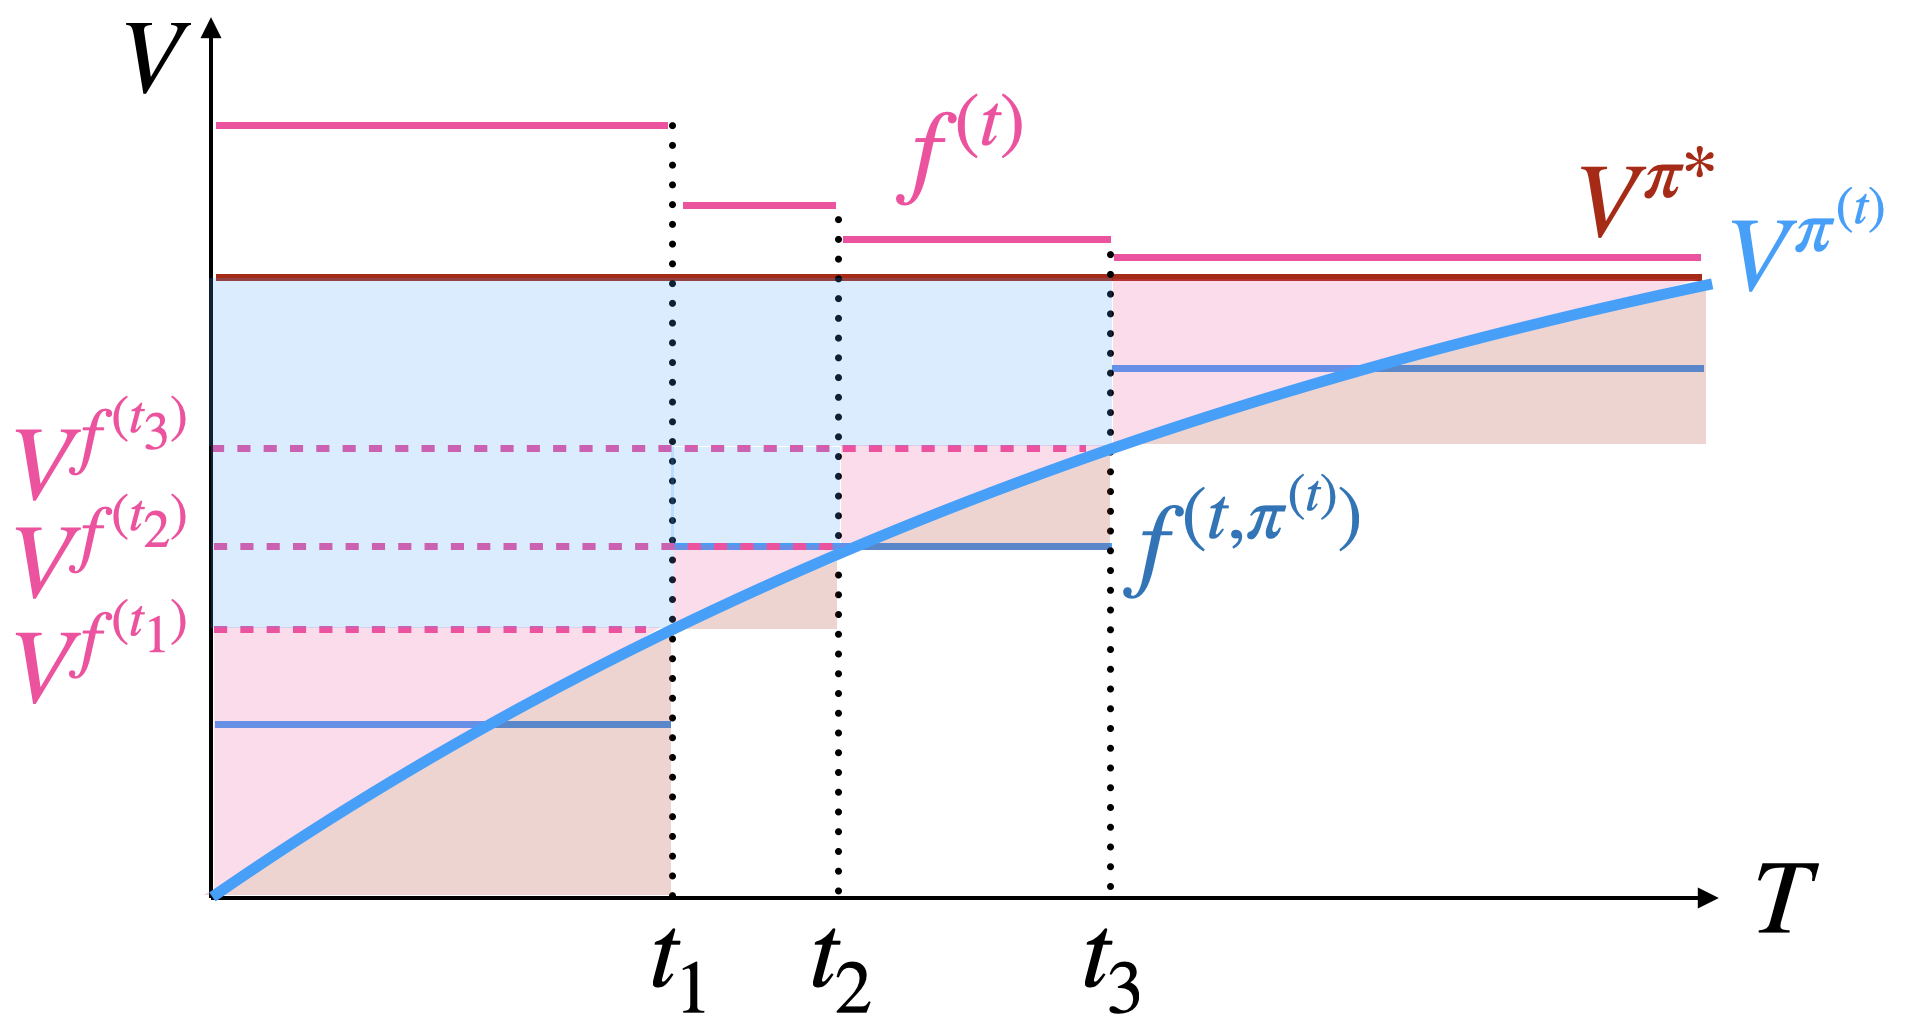
\includegraphics[width=0.5\linewidth]{figures/ch04/imgs/ac/ac_illustration.png}
    \caption[Tracking error geometry under rare-switching critics]{Illustration of tracking error in policy optimization, with a rare-switching critic $f^{(t)}$ that targets $\pi^*$. The \{blue and pink, pink\} area depicts the tracking error of \{$\pi^*$ \text{to} $\pi^{(t)}$, $\pi^{f^{(t)}}$ \text{to}  $\pi^{(t)}$\}. Both incur $\sqrt{T}$ regret. In contrast, $f^{(t,\pi^{(t)})}$ is a rare-switching critic that targets $\pi^{(t)}$, and so is insufficiently optimistic as $\pi^{(t)}$ changes. The blue, pink, and rust area depicts the tracking error of $\pi^{*}$ \text{to}  $\pi^{(t_{\last})}$ from insufficient optimism, which yields linear regret.}
    \label{fig:ac-illustration}
\end{figure}

\paragraph{A way forward.} Having the critic target $Q^*$ instead of $Q^{\pi^{(t)}}$ provides a solution. This ensures sufficient optimism, as we show in Lemma \ref{lem:ac-loss-bounded-optimism} that $f_h^{(t)} \geq \gT_h^{\pi^{(t)}}f_{h+1}^{(t)}$. Furthermore, we do not need to control $\log \mathcal{N}_{\left(\mathcal{T}^{\Pi}\right)^T \mathcal{F}}(\rho)$, as $\max_a Q_{h+1}(s,a)$ is a contraction and it suffices to control $\log \mathcal{N}_{\mathcal{T} \mathcal{F}}(\rho)$, which is often approximately $\log \mathcal{N}_{\mathcal{F}}(\rho)$. 

However, this introduces an additional term we need to control -- the deviation of the current policy $\pi^{(t)}$ from the greedy policy $\pi^{f^{(t)}}$, depicted as the pink area in Figure \ref{fig:ac-illustration}. This term is difficult to control, as $\pi^{f^{(t)}}$ changes with every critic update, and the actor requires sufficient time to catch up to the critic updates. 
To address this issue, we introduce policy resets at every critic update, allowing us to bound this with the standard mirror descent regret bound as in Lemma \ref{lem:policy-tracking-ft-t-nora}. 
The total tracking error scales with the number of critic updates -- which is then resolved by performing rare-switching critic updates in line with \citet{xiong2023generalframeworksequentialdecisionmaking}. 
% Controlling the number of critic updates is not an issue when the critic targets $Q^*$, as the Bellman operator is now the same at every iteration. 
Lastly, we increase the learning rate to reduce the regret incurred by the policy resets. This makes more aggressive policy updates to catch up with the sudden, rare, and large critic updates. 


\paragraph{Summary. } Algorithm \ref{alg:NORA} combines \emph{optimism} for strategic exploration and \emph{off-policy learning} for sample efficiency. While rare-switching critic updates are a-priori appealing, they are unstable when the critic targets $\pi^{(t)}$, due to limited optimism and the challenge of tracking a moving policy (as we describe below, and further show in Appendix \ref{app:problem-target-q-pi}). These are resolved by \emph{targeting $\pi^*$} and re-introducing \emph{rare-switching critic updates} respectively. However, this introduces additional error, as the agent has to effectively unlearn the policy after each rare critic update. We therefore introduce \emph{policy resets} to the uniform policy after each critic update -- incurring minimal cost due to their rarity (as there are only $O(dH\log T)$ updates). A \emph{more aggressive learning rate} (by a factor of $\sqrt{dH\log T}$) mitigates some of the additional regret incurred, and can be seen as making more aggressive updates to make up for lost ground from policy resets. See Appendix \ref{app:proof-nora} for more details.

\begin{algorithm}[t]
    \caption{\aigen{Rare-Switching Optimistic Actor-Critic with Uniform Actor Resets}}
    \begin{algorithmic}[1]
            \STATE {\bfseries Input:} Function class $\gF$.
            \STATE {\bfseries Initialize:} $\gF^{(0)} \leftarrow \gF$, offline dataset $\gD_{\off}$, $\gD_h^{(0)}\leftarrow \emptyset, \forall h \in [H]$, $\eta = \Theta(\sqrt{d\log T \log|\gA| H^{-1}T^{-1}})$, $\pi^{(1)} \; \propto \; 1$, confidence width $\beta=\Theta(\log (HT^2 \mathcal{N}_{\gF, \gT \gF}(1/T) / \delta))$.
            \FOR{episode $t = 1, 2, \dots, T$}
            \STATE Set $f_h^{(t)}(s,a) \in \operatorname{argmax}_{f \in \mathcal{F}^{(t_{\text{last}})}} f_h\left(s,a\right) \forall s,a,h$.
            \STATE Play policy $\pi^{(t)}$ for one episode, obtain trajectory, update dataset $\mathcal{D}_h^{(t)}$. \IF{$\mathcal{L}_h^{(t)}(f_h^{(t)}, f_{h+1}^{(t)}) \geq \min_{f_h' \in \gF_h} \mathcal{L}_h^{(t)}(f_h', f_{h+1}^{(t)}) + 5H^2\beta$ for some $h$} %$m^{(t-1)} \leq \widehat{c}_{\on}^{(t)} - 1$
            \STATE Compute confidence set $\gF^{(t)}$:
            \begingroup
            \addtolength\jot{-1ex}
            \begin{align*}
                &\mathcal{F}^{(t)} \leftarrow\left\{f \in \mathcal{F}: \mathcal{L}_h^{(t)}\left(f_h, f_{h+1}\right)-\min _{f_h^{\prime} \in \mathcal{F}_h} \mathcal{L}_h^{(t)}\left(f_h^{\prime}, f_{h+1}\right) \leq H^2\beta \; \forall h\right\},\\
                &\mathcal{L}_h^{(t)}\left(f, f'\right) \gets\sum_{\left(s, a, r, s^{\prime}\right) \in \mathcal{D}_h^{(t)}}\left(f(s, a)-r-\max_{a' \in \gA}f^{\prime}(s^{\prime}, a')\right)^2.
            \end{align*}
            \endgroup
            \STATE Reset policy $\pi^{(t)} \; \propto \; 1$. 
            \STATE Set $t_{\text{last}} \gets t$, $N_{\text{updates}}^{(t)} \gets N_{\text{updates}}^{(t-1)}+ 1$.
            \ELSE
            \STATE Set $N_{\text{updates}}^{(t)} \gets N_{\text{updates}}^{(t-1)}$, $\gF^{(t)} \gets \gF^{(t-1)}$.
            \ENDIF
        \STATE Update $\pi_h^{(t+1)}(a|s) \; \propto \; \pi_h^{(t)}(a|s)\exp(\eta f_h^{(t)}(s,a))$.
        \ENDFOR
    \end{algorithmic}
\label{alg:NORA}
\end{algorithm}



% The above algorithm amounts to maintaining an actor updated with policy gradient updates alongside the GOLF critic from \citet{xie2022role}, while incorporating hybrid data into the critic estimation in the same vein as \citet{tan2024natural}. Note that although the policy changes in every episode, we can show that the covering number of the value function class only increases in the number of critic updates, and not the number of policy updates. We write $\mathcal{L}_h^{(t_1:t_2, \pi)}\left(f, f^{\prime}\right):=\sum_{\left(s, a, r, s^{\prime}\right) \in \mathcal{D}_h^{(t_2)}\setminus \mathcal{D}_h^{(t_1)}}\left(f(s, a)-r-f^{\prime}(s^{\prime}, \pi_{h+1}(s'))\right)^2$, and use the shorthand $\gL_h^{\left(1:t,\pi^{f^{(t)}}\right)} = \gL_h^{(t)}$.

% That is, we update the critic when the cumulative temporal difference (TD) loss exceeds a certain threshold. If we used the TD loss with respect to the current policy, large changes in the policy may cause correspondingly large changes in the TD loss, 


\section{Regret bound for rare-switching optimistic actor-critic}


To control the switching cost with the framework of \citet{xiong2023generalframeworksequentialdecisionmaking}, we concern ourselves with function classes of low $D_\Delta$-type Bellman Eluder dimension \citep{jin2021bellmaneluder}:

\begin{aspt}[Bounded $D_{\Delta}$-type Bellman Eluder Dimension]
    Let $\mathcal{D}_{\Delta}:=\left\{\mathcal{D}_{\Delta, h}\right\}_{h \in[H]}$, where $\mathcal{D}_{\Delta, h}=\left\{\delta_{(s, a)}(\cdot) \mid s \in \mathcal{S}, a \in \mathcal{A}\right\}$. That is, we only consider distributions that are Dirac deltas on a single state-action pair. We assume that $d := d_{\text{BE}}(\gF, D_\Delta, 1/\sqrt{T}) < \infty$. 
\end{aspt}

This can be weakened to the more general $\ell_2$ eluder condition of \cite{xiong2023generalframeworksequentialdecisionmaking} with nothing more than a change in notation. However, we present our results in the Bellman eluder dimension framework for familiarity and ease of presentation. We now show the following for Algorithm \ref{alg:NORA}:

\begin{thm}[Regret Bound for \aigen{Algorithm~\ref{alg:NORA}}]
\label{thm:nora-regret_bound}
Algorithm \ref{alg:NORA} achieves the following regret with probability at least $1-\delta$:
\begin{align}
    \mathrm{Reg}(T)
    &= O\left(\sqrt{d H^5 T \log T \log|\gA|} + dH^3 \log T + \sqrt{\beta H^4 T  \mathsf{SEC}(\gF, \Pi, T)}\right).
\end{align}
where $\beta = \Theta(\log \left(HT^2 \mathcal{N}_{\gF,\gT \gF}(1/T) / \delta\right) )$.
This implies a sample complexity (ignoring lower-order terms) of 
\begin{align}N \geq \Omega\left(dH^5 \log T\log|\gA|/\epsilon^2 + H^4 \beta \mathsf{SEC}(\gF, \Pi, T)/\epsilon^2\right).\end{align}
\end{thm}

\begin{proof}[Proof sketch:]
%    We provide a proof sketch here, and defer the full proof to Appendix \ref{app:proof-nora}. 
By Lemma \ref{lem:regret-decomp-ac}, we have a slightly different regret decomposition than usual:
    \begin{align}\label{eqn:nora-regret-decom}
    \operatorname{Reg}(T)
    = & \underbrace{\sum_{t=1}^T \sum_{h=1}^H \mathbb{E}_{\pi^*}\left[\left\langle f_h^{(t)}\left(s_h, \cdot\right), \pi_h^*\left(\cdot \mid s_h\right)-\pi_h^{(t)}\left(\cdot \mid s_h\right)\right\rangle\right]}_{\text{\textcolor{red}{Tracking error of $\pi^{(t)}$ w.r.t. $\pi^*$, bounded by mirror ascent arguments.}}} \nonumber\\ 
    &\qquad\underbrace{-\sum_{t=1}^T \sum_{h=1}^H\mathbb{E}_{\pi^*}\left[\left(f_h^{(t)}-\gT_h^{\pi^{*}}f_{h+1}^{(t)}\right)\left(s_h, a_h\right)\right]}_{\text{\textcolor{orange}{Negative Bellman error under $\pi^*$, bounded by optimism.}}} \nonumber\\
    &\qquad\underbrace{+ \sum_{t=1}^T \sum_{h=1}^H\mathbb{E}_{\pi^{(t)}}\left[\left(f_h^{(t)}-\gT_h f_{h+1}^{(t)}\right)\left(s_h, a_h\right)\right]}_{\text{\textcolor{blue}{Bellman error under current policy occupancy, bounded by critic error.}}}\nonumber\\
    &\underbrace{+\sum_{t=1}^T \sum_{h=1}^H \mathbb{E}_{\pi^{(t)}}\left[\left\langle f_{h+1}^{(t)}(s', \cdot), \pi_{h+1}^{f^{(t)}}(\cdot | s')-\pi_{h+1}^{(t)}(\cdot | s')\right\rangle\right]}_{\text{\textcolor{teal}{Tracking error of $\pi^{(t)}$ w.r.t. $\pi^{f^{(t)}}$, bounded by mirror ascent and policy resets.}}}.
\end{align}

 We will then bound each term in (\ref{eqn:nora-regret-decom}) separately. We further decompose the first term as follows
 \begin{align}\label{eqn:nora-regret-decom-1}
           &\sum_{t=1}^T \sum_{h=1}^H \mathbb{E}_{\pi^{(t)}}\left[\left\langle f_h^{(t)}\left(s_{h+1}, \cdot\right), \pi_{h+1}^{\star}\left(\cdot \mid s_{h+1}\right)-\pi_{h+1}^{(t)}\left(\cdot \mid s_h\right)\right\rangle\right] \nonumber\\
        &= \sum_{k=1}^{K} \sum_{t=t_{k}+1}^{t_{k+1}} \sum_{h=1}^H \mathbb{E}_{\pi^{(t)}}\left[\left\langle f_h^{(t)}\left(s_h, \cdot\right), \pi_h^{\star}\left(\cdot \mid s_h\right)-\pi_h^{(t)}\left(\cdot \mid s_h\right)\right\rangle\right] \nonumber\\
        &= \sum_{k=1}^{K} \sum_{t=t_{k}+1}^{t_{k+1}-1} \sum_{h=1}^H \mathbb{E}_{\pi^{(t)}}\left[\left\langle f_h^{(t)}\left(s_h, \cdot\right), \pi_h^{\star}\left(\cdot \mid s_h\right)-\pi_h^{(t)}\left(\cdot \mid s_h\right)\right\rangle\right] \nonumber\\
        &\qquad+ \sum_{k=1}^{K}\sum_{h=1}^H \mathbb{E}_{\pi^{(t)}}\left[\left\langle f_h^{(t_k)}\left(s_h, \cdot\right), \pi_h^{\star}\left(\cdot \mid s_h\right)-\pi_h^{(t_k)}\left(\cdot \mid s_h\right)\right\rangle\right].
 \end{align}
For the first term of (\ref{eqn:nora-regret-decom-1}), following Lemma \ref{lem:mirror-descent-nora} and summing over all $t_1,\ldots,t_K$, we have
\begin{align}\label{eqn:nora-regret-decom-11}
    \sum_{k=1}^{K}\sum_{t=t_k+1}^{t_{k+1}-1} \sum_{h=1}^H \mathbb{E}_{\pi^*}\left[\left\langle f_h^{(t)}\left(s_h, \cdot\right), \pi_h^*\left(\cdot \mid s_h\right)-\pi_h^{(t)}\left(\cdot \mid s_h\right)\right\rangle\right] \leq \eta H^3 T/2 + \frac{KH \log |\gA|}{\eta} + KH^2,
\end{align}
 while for the second term, one may note that each inner product can be bounded by $2H$, therefore the summation can be bounded as
 \begin{align}\label{eqn:nora-regret-decom-12}
   \sum_{k=1}^{K}\sum_{h=1}^H \mathbb{E}_{\pi^{(t)}}\left[\left\langle f_h^{(t_k)}\left(s_h, \cdot\right), \pi_h^{\star}\left(\cdot \mid s_h\right)-\pi_h^{(t_k)}\left(\cdot \mid s_h\right)\right\rangle\right]\leq 2KH^2.
 \end{align}
 We apply this similar strategy on the fourth term of (\ref{eqn:nora-regret-decom}), which leads to the following decomposition
 \begin{align}\label{eqn:nora-regret-decom-4}
     &\sum_{t=1}^T \sum_{h=1}^H \mathbb{E}_{\pi^{(t)}}\left[\left\langle f_h^{(t)}\left(s_{h+1}, \cdot\right), \pi_{h+1}^{f^{(t)}}\left(\cdot \mid s_{h+1}\right)-\pi_{h+1}^{(t)}\left(\cdot \mid s_h\right)\right\rangle\right] \nonumber\\
 %       &= \sum_{k=1}^{K} \sum_{t=t_{k}+1}^{t_{k+1}} \sum_{h=1}^H \mathbb{E}_{\pi^{(t)}}\left[\left\langle f_h^{(t)}\left(s_h, \cdot\right), \pi_h^{f^{(t)}}\left(\cdot \mid s_h\right)-\pi_h^{(t)}\left(\cdot \mid s_h\right)\right\rangle\right] \nonumber\\
        &= \sum_{k=1}^{K} \sum_{t=t_{k}+1}^{t_{k+1}-1} \sum_{h=1}^H \mathbb{E}_{\pi^{(t)}}\left[\left\langle f_h^{(t)}\left(s_h, \cdot\right), \pi_h^{f^{(t)}}\left(\cdot \mid s_h\right)-\pi_h^{(t)}\left(\cdot \mid s_h\right)\right\rangle\right] \nonumber\\
        &\qquad+ \sum_{k=1}^{K}\sum_{h=1}^H \mathbb{E}_{\pi^{(t)}}\left[\left\langle f_h^{(t_k)}\left(s_h, \cdot\right), \pi_h^{f^{(t)}}\left(\cdot \mid s_h\right)-\pi_h^{(t_k)}\left(\cdot \mid s_h\right)\right\rangle\right],
 \end{align}
 and the first term of (\ref{eqn:nora-regret-decom-4}) is bounded by Lemma \ref{lem:policy-tracking-ft-t-nora} with summing over all $t_1,\ldots,t_K$ as
 \begin{align}\label{eqn:nora-regret-decom-41}
     \sum_{k=1}^{K}\sum_{t=t_k+1}^{t_{k+1}-1} \sum_{h=1}^H \E_{d_h^{(t)}}\left[\left\langle f_{h+1}^{(t)}(s', \cdot) , \pi_{h+1}^{f^{(t)}}(\cdot | s') - \pi_{h+1}^{(t)} (\cdot | s')\right\rangle\right] \leq \eta H^3 T/2 + \frac{KH\log|\gA|}{\eta} + KH^2,
 \end{align}
 while the second term of (\ref{eqn:nora-regret-decom-4}) can be bounded similar to (\ref{eqn:nora-regret-decom-12}) as
  \begin{align}\label{eqn:nora-regret-decom-42}
   \sum_{k=1}^{K}\sum_{h=1}^H \mathbb{E}_{\pi^{(t)}}\left[\left\langle f_h^{(t_k)}\left(s_h, \cdot\right), \pi_h^{f^{(t)}}\left(\cdot \mid s_h\right)-\pi_h^{(t_k)}\left(\cdot \mid s_h\right)\right\rangle\right]\leq 2KH^2.
 \end{align}
  It only remains to bound the second term and third term of (\ref{eqn:nora-regret-decom}). We note that targeting $Q^*$ yields sufficient optimism to assert that $f_h^{(t)} \geq \gT_h^{\pi^{*}} f_{h+1}^{(t)}$ in Lemma \ref{lem:ac-loss-bounded-optimism}, and so we argue that the second term in (\ref{eqn:nora-regret-decom}) for the negative Bellman error under $\pi^*$ is nonpositive in Lemma \ref{lem:negative-bellman-decomp},
  \begin{align}\label{eqn:nora-regret-decom-2}
   -\sum_{t=1}^T \sum_{h=1}^H\mathbb{E}_{\pi^*}\left[\left(f_h^{(t)}-\gT_h^{\pi^{*}}f_{h+1}^{(t)}\right)\left(s_h, a_h\right)\right]\leq 0
  \end{align}
  The third term via a standard argument from \citet{xie2022role} in Lemma \ref{lem:occ-measure-regret-nora},
  \begin{align}\label{eqn:nora-regret-decom-3}
      \sum_{t=1}^T \sum_{h=1}^H\mathbb{E}_{\pi^{(t)}}\left[\left(f_h^{(t)}-\gT_h f_{h+1}^{(t)}\right)\left(s_h, a_h\right)\right] \leq \sqrt{\beta H^4 T\mathsf{SEC}(\gF, \Pi, T)}.
  \end{align}
Plugging (\ref{eqn:nora-regret-decom-1}) -- (\ref{eqn:nora-regret-decom-3}) into (\ref{eqn:nora-regret-decom}), we obtain that
\begin{align}
    \mathrm{Reg}(T) &\leq \eta H^3 T + \frac{2KH\log|\gA|}{\eta} + 6KH^2 + \sqrt{\beta H^4 T\mathsf{SEC}(\gF, \Pi, T)} \nonumber\\
    & \leq \eta H^3 T +  \frac{2dH^2\log T\log|\gA|}{\eta} + 6dH^3\log T +  \sqrt{\beta H^4 T\mathsf{SEC}(\gF, \Pi, T)}\nonumber\\
    & = 2\sqrt{2dH^5T\log T\log|\gA|} +6dH^3\log T +  \sqrt{\beta H^4 T\mathsf{SEC}(\gF, \Pi, T)}
\end{align}
 %Instead of directly bounding the first and fourth terms right away, consider the critic switch times $t_1,...,t_K$. Then,
 %$$\sum_{t=t_k+1}^{t_{k+1}} \sum_{h=1}^H \mathbb{E}_{\pi^{(t)}}\left[\left\langle f_{h+1}^{(t)}(s', \cdot), \pi_{h+1}^{f^{(t)}}(\cdot | s')-\pi_{h+1}^{(t)}(\cdot | s')\right\rangle\right]$$
 %is bounded by $O(\eta H^3(t_{k+1} - t_k) + H\log|\gA|/\eta + H^2)$ in Lemma \ref{lem:policy-tracking-ft-t-nora}. We exploit the fact that we reset the policy after the episode is collected at every $t_k$ in doing so. We do the same for the other term in Lemma \ref{lem:mirror-descent-nora}. 
 where the second inequality is obtained by bounding the number of critic updates by $dH\log T$ in Lemma \ref{lem:switch-cost} with the techniques of \citet{xiong2023generalframeworksequentialdecisionmaking}, and the last equality holds when we set the learning rate $\eta = \Theta(\sqrt{d\log T \log |\gA| H^{-1}T^{-1}})$. Here we conclude the proof.
 %Summing over all $t_1,...,t_K$ lets us bound the first and fourth terms by $\sqrt{dH^5\log T\log|\gA|} + dH^3 \log T$ by our choice of learning rate. We modify the learning rate $\eta = \Theta(\sqrt{d\log T \log |\gA| H^{-1}T^{-1}})$ to mitigate the switch cost, shaving off a factor of $dH\log T$ in the final sample complexity. Putting everything together yields the result.
\end{proof}

\paragraph{Quality of the regret bound.} 
% This regret bound is very encouraging. 
Even compared to the ``good case'' for Algorithm \ref{alg:DOUHUA} in Corollary \ref{cor:good-case-douhua}, Algorithm \ref{alg:NORA} requires only $dH \log T$ more samples to learn an $\epsilon$-optimal policy. This is exactly the same as the switch cost, in line with what \citet{cassel2024warm} observed for linear MDPs. 


It is known that the Bellman eluder dimension may scale unfavorably with $T$ in rare cases \citep{xie2022role} where $d = d_{\text{BE}}(\gF, D_\Delta, 1/\sqrt{T}) = \Omega(\sqrt{T})$. Although we use the $\mathsf{SEC}$ of \citet{xie2022role} to bound the online regret whenever possible, as it is never larger than $O(d\log T)$, our result still depends on $d$ due to the switch cost. Still, function classes with low Bellman eluder dimension are ubiquitous, and so Algorithm \ref{alg:NORA} achieves $\sqrt{T}$ regret on a large class of problems including linear and kernel MDPs \citep{jin2021bellmaneluder}. We note that it is possible to weaken the dependence on the $d_\Delta$-type Bellman eluder dimension to the $\ell_2$ eluder condition of \cite{xiong2023generalframeworksequentialdecisionmaking} with nothing more than a change of notation, but we present our results in the language of the Bellman eluder dimension for ease of presentation.


\paragraph{Comparison with prior work.} The only other method we know of that claims to have achieved $\sqrt{T}$ regret with policy optimization and general function approximation is \citet{zhou2023offline}. However, they allow themselves to collect $\Omega(T)$ samples \textit{at every timestep $t$ without incurring any additional regret}. This incurs a sample complexity of $1/\epsilon^6$, while Algorithm \ref{alg:NORA} enjoys a $1/\epsilon^2$ guarantee in comparison. As such, their regret bound is not sublinear in the more common setup where this sampling contributes to the regret. 
\citet{liu2023optimistic} achieve a result of $1/\epsilon^3$ by performing critic updates in batches. However, \citet{liu2023optimistic} do not account for the potential growth of the policy class in the $O(\sqrt{T})$ critic updates they make. Their result of $1/\epsilon^3$ sample complexity is therefore somewhat optimistic, and may very well be $1/\epsilon^4$. 



% \kevin{Likely that the rare-switching will come up when we have to prove this lemma. Abbasi-Yadkori et al (2011) bound the regret with the inflation factor coming up in the change of determinants, $\det(V_t) < (1+C)\det(V_{\tau_t})$ in Appendix D. This amounts to showing that the prediction error is off by at most a constant. The regret is therefore only inflated by a $(1+C)$-factor. For us, we can similarly show that the Bellman error is inflated by at most a constant when performing rare-switching updates, because between updates the cumulative Bellman error does not change much. }


% \paragraph{Targeting $Q^*$.} Targeting $Q^{\pi^{(t)}}$ instead of $Q^*$ immediately poses an issue. It can be shown, and we do so in Lemma \ref{lem:b2-covering-number-policy}, that the covering number of the value function class:
% $$\gV_h = \left\{\left\langle f_h(s, \cdot), \pi_h(\cdot | s)\right\rangle \mid f_h \in \gF_h, \pi \in \Pi\right\},$$
% containing value function estimates with regard to stochastic policies $\pi$ has a log-covering number that grows linearly with regard to the number of critic updates. Previously, in \citet{zhong2023theoretical}, it was thought that this increases with the number of policy and critic updates. Although we tighten this dependence to only the latter, this immediately implies that a rare-switching critic update is essential to achieving optimal sample complexity.



% \begin{aspt}[Policy Augmented Generalized Completeness]
%     There exists an auxiliary function class $\gG = \gG_1 \times ...\times\gG_H$ such that $g_h : \gS \times \gA \to [0,H]$ for all $g_h \in \gG_h$, that is rich enough such that for all $f_{h+1} \in \gF_{h+1}$ and all $\pi\in \Pi$, $\gT_h^\pi f_{h+1} \in \gG_h$. 
% \end{aspt}


\paragraph{Extension to other policy updates.} We are able to accommodate other policy optimization updates other than the multiplicative weights update, if they satisfy the following:

\begin{cor}
    If there exists some policy optimization oracle $\pi^{(t+1)} \gets \mathrm{PO}(\pi^{(t)}, f^{(t)}, \eta)$ and some $\mathrm{OPT}^*$ and $\mathrm{OPT}^f$ such that
    \begin{subequations}
    \begin{align}
        &\sum_{t=1}^T \sum_{h=1}^H \mathbb{E}_{\pi^*}\left[\left\langle f_h^{(t)}(s, \cdot), \pi_h^*(\cdot | s)-\pi_h^{(t)}(\cdot | s)\right\rangle\right] \leq \mathrm{OPT}^*,\\
    &\sum_{t=1}^T \sum_{h=1}^H \mathbb{E}_{\pi^{(t)}}\left[\left\langle f_h^{(t)}(s, \cdot), \pi_h^{f^{(t)}}(\cdot | s)-\pi_h^{(t)}(\cdot | s)\right\rangle\right] \leq \mathrm{OPT}^f,
    \end{align}
    \end{subequations}
    then Algorithm \ref{alg:NORA} with this policy update obtains a regret of
    \begin{equation}\mathrm{Reg}(T) = O\left(\sqrt{\beta H^4 T \mathsf{SEC}(\gF, \Pi, T)} + \mathrm{OPT}^* + \mathrm{OPT}^f\right).\end{equation}
\end{cor}


\section{Connections to deep actor-critic methods}


\paragraph{Targeting $Q^*$.} We are not the only ones who consider a critic that targets $Q^*$ instead of $Q^{\pi^{(t)}}$. By way of illustration, \citet{crites1994actorcriticqlearning} propose an actor-critic algorithm that mimics Q-learning via a critic that targets $Q^*$. Another example is the popular DDPG algorithm \citep{lillicrap2015continuous} and its successor, TD3 \citep{fujimoto2018addressing}, that take turns to update an approximately greedy deterministic policy that approximately maximizes an estimate of the approximately greedy deterministic policy's Q-function (and so approximately targets $Q^*$), while performing stochastic exploration that tracks the deterministic policy over time. 
% We elaborate on the spiritual similarities between Algorithm \ref{alg:NORA} and DDPG later in this section.

\paragraph{Similarity to deep deterministic policy gradients (DDPG).} Several aspects of the design of Algorithm \ref{alg:NORA} are reminiscent of the popular DDPG algorithm of \citet{lillicrap2015continuous}. DDPG alternates between optimizing a deterministic policy $g_h^{(t)}(s)$ and a critic $f_h^{(t)}(s,a)$:
\begin{align}
    g_h^{(t)}(s) &\approx \argmax_{a\in\gA} f_h^{(t)}(s,a), \\
    f_h^{(t)}(s,a) &\approx \argmin \gL_h^{(t,g^{(t-k)})}(f_h,f_{h+1}^{(t-k)}),
    \label{eqn:ddpg}
\end{align}
while exploring according to a stochastic exploration policy that tracks the deterministic policy. In practice, the exploration policy $\pi_{\text{exp}}^{(t)}(a|s) \propto \mathbbm{1}(a = g^{(t)}(s)) + \gN_t$ is often given by the deterministic function perturbed by Gaussian noise. The critic is optimized according to slowly updating targets approximating the actor and critic from a few steps ago -- in a manner reminiscent of the rare-switching critic update in Algorithm \ref{alg:NORA}. As the deterministic policy approximates the greedy policy, and the approximately greedy policy is used when computing TD error targets, the DDPG critic approximately targets $Q^*$. This suggests that DDPG and its successor TD3 \citep{fujimoto2018addressing} may be useful backbones for adapting algorithmic insights garnered from the design and analysis of Algorithm \ref{alg:NORA} for practical RL.\footnote{This provides insight on why DDPG/TD3 are more sample-efficient than on-policy PPO. Algorithm \ref{alg:NORA} needs $1/\epsilon^2$ samples, while on-policy sampling needs at least $1/\epsilon^4$ \citep{liu2023optimistic}} 


\section{Extension to hybrid RL}
\label{sec:hybrid-rl}

In this section, we demonstrate that the benefits of having access to both offline and online data are two-fold with actor-critic algorithms. With optimism, actor-critic algorithms achieve sample efficiency gains. However, if one does not wish to use an optimistic algorithm (as optimism is difficult to implement in practice with deep function approximation), having access to offline data allows one to omit the use of optimism, achieving computational efficiency gains \citep[e.g.,][]{jin2021pessimism, li2024settling, rashidinejad2021bridging}. 

% Before we proceed, it is useful to introduce the partial all-policy concentrability coefficient from \citet{tan2024natural}.
% \begin{defn}[Partial All-Policy Concentrability Coefficient]
%     For a function class $\gF$ and a partition on the state-action space $\gX = \gS \times \gA \times [H]$, where we denote the offline and online partitions by $\gX_{\off}$ and $\gX_{\on}$, respectively, the partial all-policy concentrability coefficient is given by:
%     \begin{align*}
%     c_{\off}(\gF\mathbbm{1}_{\gX_{\off}}) 
%     &\coloneqq \max_h \sup_{f \in \gF} \frac{\|(f_h - \gT_h f_{h+1}) \mathbbm{1}_{(\cdot, h) \in \gX_{\off}}\|_{2, d_h^\pi}^2}{\|(f_h - \gT_h f_{h+1})\mathbbm{1}_{(\cdot, h) \in \gX_{\off}}\|_{2, \mu_{h}}^2},
%     \end{align*}
%     where $\mathbbm{1}_{\gX_{\off}}$ denotes the indicator variable for whether $s,a\in \gX_{\on}.$
%     \label{defn:partial-all-policy-concentrability}
% \end{defn}

% \begin{defn}[Single-Policy Concentrability Coefficient]
%     $$c_{\off}^*(\gF,\Pi) = \max_{h\in[H]}\sup_{f \in \gF} \sup_{\pi \in \Pi} \frac{\E_{\pi^*}\left[f_h-\gT_h^{\pi}f_{h+1} \right]^2}{\E_{\mu}[\left(f_h-\gT_h^{\pi}f_{h+1}\right)^2]}, \;\; c_{\off}^*(\gF) = \max_{h\in[H]}\sup_{f \in \gF} \frac{\E_{\pi^*}\left[f_h-\gT_h f_{h+1} \right]^2}{\E_{\mu}[\left(f_h-\gT_h f_{h+1}\right)^2]}.$$
%     \label{defn:single-policy-concentrability}
% \end{defn}

\section{Computational efficiency through optimism-free hybrid RL}

The benefits of hybrid RL extend beyond sample efficiency gains. \citet{song2023hybrid, amortila2024harnessing, zhou2023offline} show that it is possible for a hybrid RL algorithm to bypass the need for optimism altogether, as long as the offline dataset achieves sufficient coverage. In this spirit, we provide \aigen{two non-optimistic hybrid actor-critic variants} in Algorithms \ref{alg:NOAH-pi} and \ref{alg:NOAH-star} that achieve $\sqrt{T}$ regret without using optimism. Algorithm \ref{alg:NOAH-pi} targets $\pi^{(t)}$, and follows the very natural procedure of performing a critic update via Fitted Q-Evaluation (FQE) \citep{munos2008finite} and an actor update in every episode. It therefore requires closure of the critic function class under truncated sums as in Definition \ref{defn:closure-truncated-sums} to control the growth of the policy class as in Lemma \ref{lem:policy-class-growth-sums}. Algorithm \ref{alg:NOAH-star}, like \aigen{Algorithm~\ref{alg:NORA}}, circumvents this by targeting $\pi^*$ and performing a rare-switching critic update. Both algorithms are fully off-policy, utilizing offline data and all collected online data without throwing any away. 

We use the following form of the single-policy concentrability coefficient, tweaked from that of \citet{zhan2022offline}, that has some resemblance to the transfer coefficient of \cite{song2023hybrid}:
\begin{defn}[Single-Policy Concentrability Coefficient]
    $$c_{\off}^*(\gF,\Pi) = \max_{h\in[H]}\sup_{f \in \gF} \sup_{\pi \in \Pi} \frac{\E_{\pi^*}\left[f_h-\gT_h^{\pi}f_{h+1} \right]^2}{\E_{\mu}[\left(f_h-\gT_h^{\pi}f_{h+1}\right)^2]}, \;\; c_{\off}^*(\gF) = \max_{h\in[H]}\sup_{f \in \gF} \frac{\E_{\pi^*}\left[f_h-\gT_h f_{h+1} \right]^2}{\E_{\mu}[\left(f_h-\gT_h f_{h+1}\right)^2]}.$$
    \label{defn:single-policy-concentrability}
\end{defn}
Notably, this is similar to the squared Bellman error variant of the single policy concentrability coefficient in the literature, with the exception that the square in the numerator is outside the expectation, and we have an additional supremum over policies that the Bellman operator is taken with respect to in the first definition. 

With the definition of single-policy concentrability coefficient, we provide a guarantee for this procedure below, but defer the proof to Appendices \ref{app:noah-pi-proofs} and \ref{app:noah-star-proofs}. At a high level, the proofs proceed in a similar way to Theorems \ref{thm:regret-bound-douhua} and \ref{thm:nora-regret_bound}, with the exception that the negative Bellman error under $\pi^*$ is bounded using the critic's Bellman error under the offline data. 



\begin{algorithm}[t]
    \caption{\aigen{Non-Optimistic Hybrid Actor-Critic Targeting $\pi^{(t)}$}}
    \begin{algorithmic}[1]
            \STATE {\bfseries Input:} Function class $\gF$.
            \STATE {\bfseries Initialize:} $\gF^{(0)} \leftarrow \gF$, $\gD_h^{(0)}\leftarrow \emptyset, \forall h \in [H]$, $\eta = \Theta(\sqrt{\log|\gA| H^{-2}T^{-1}})$, $\pi^{(1)} \; \propto \; 1$, confidence width $\beta=\Theta(\log (HT^2 \mathcal{N}_{\gF, \gT \gF}(1/T) / \delta))$.
            \FOR{episode $t = 1, 2, \dots, T$}
            \STATE Play policy $\pi^{(t)}$ for one episode, obtain trajectory, update dataset $\mathcal{D}_h^{(t)}$. 
            \STATE Compute critic $f^{(t+1)}$ targeting $\pi^{(t)}$ via FQE:
            \begingroup
            \addtolength\jot{-1ex}
            \begin{align*}
                &f^{(t)} \leftarrow \argmin_{f \in \gF} \mathcal{L}_h^{(t,\pi^{(t)})}\left(f_h, f_{h+1}\right) \text{ for } h=H-1,...,1,\\
                &\mathcal{L}_h^{(t, \pi^{(t)})}\left(f, f'\right) \gets\sum_{\left(s, a, r, s^{\prime}\right) \in \mathcal{D}_h^{(t)}\cup\gD_{\off}}\left(f(s, a)-r-f^{\prime}(s^{\prime}, \pi_{h+1}^{(t)}(s^\prime))\right)^2.
            \end{align*}
            \endgroup
        \STATE Update $\pi_h^{(t+1)}(a|s) \; \propto \; \pi_h^{(t)}(a|s)\exp(\eta f_h^{(t)}(s,a))$.
        \ENDFOR
    \end{algorithmic}
\label{alg:NOAH-pi}
\end{algorithm}


\begin{algorithm}[t]
    \caption{\aigen{Non-Optimistic Hybrid Actor-Critic Targeting $\pi^*$}}
    \begin{algorithmic}[1]
            \STATE {\bfseries Input:} Function class $\gF$.
            \STATE {\bfseries Initialize:} $\gF^{(0)} \leftarrow \gF$, $\gD_h^{(0)}\leftarrow \emptyset, \forall h \in [H]$, $\eta = \Theta(\sqrt{d\log T \log|\gA| H^{-1}T^{-1}})$, $\pi^{(1)} \; \propto \; 1$, confidence width $\beta=\Theta(\log (HT^2 \mathcal{N}_{\gF, \gT \gF}(1/T) / \delta))$.
            \FOR{episode $t = 1, 2, \dots, T$}
            \STATE Play policy $\pi^{(t)}$ for one episode, obtain trajectory, update dataset $\mathcal{D}_h^{(t)}$. \IF{$\mathcal{L}_h^{(t)}(f_h^{(t)}, f_{h+1}^{(t)}) \geq \min_{f_h' \in \gF_h} \mathcal{L}_h^{(t)}(f_h', f_{h+1}^{(t)}) + 5H^2\beta$ for some $h$} %$m^{(t-1)} \leq \widehat{c}_{\on}^{(t)} - 1$
            \STATE Compute critic $f^{(t+1)}$ via FQE:
            \begingroup
            \addtolength\jot{-1ex}
            \begin{align*}
                &f^{(t)} \leftarrow \argmin_{f \in \gF} \mathcal{L}_h^{(t)}\left(f_h, f_{h+1}\right) \text{ for } h=H-1,...,1,\\
                &\mathcal{L}_h^{(t)}\left(f, f'\right) \gets\sum_{\left(s, a, r, s^{\prime}\right) \in \mathcal{D}_h^{(t)}\cup\gD_{\off}}\left(f(s, a)-r-\max_{a' \in \gA}f^{\prime}(s^{\prime}, a')\right)^2.
            \end{align*}
            \endgroup
            \STATE Reset policy $\pi^{(t)} \; \propto \; 1$. 
            \STATE Set $t_{\text{last}} \gets t$, $N_{\text{updates}}^{(t)} \gets N_{\text{updates}}^{(t-1)}+ 1$.
            \ELSE
            \STATE Set $N_{\text{updates}}^{(t)} \gets N_{\text{updates}}^{(t-1)}$, $f^{(t+1)} \gets f^{(t)}$.
            \ENDIF
        \STATE Update $\pi_h^{(t+1)}(a|s) \; \propto \; \pi_h^{(t)}(a|s)\exp(\eta f_h^{(t)}(s,a))$.
        \ENDFOR
    \end{algorithmic}
\label{alg:NOAH-star}
\end{algorithm}


\begin{thm}[Regret Guarantee of Algorithm \ref{alg:NOAH-pi}]
    Let $c_{\off}^*(\gF,\Pi)$ be the single-policy concentrability coefficient defined in Definition \ref{defn:single-policy-concentrability}. Algorithm~\ref{alg:NOAH-pi} satisfies with probability at least $1-\delta$:
    \begin{align}
        \mathrm{Reg}^\pi(T)
        = O\left(\sqrt{H^4 T \log|\gA|} + \sqrt{\beta^\pi H^4 c_{\off}^*(\gF,\Pi)T^2/N_{\off}} + \sqrt{\beta^\pi H^4 T\mathsf{SEC}(\gF, \Pi, T)}\right).
    %    \mathrm{Reg}^*(T)
    %    &= O\left(\sqrt{d H^5 T \log T \log|\gA|} + dH^3 \log T + \sqrt{\beta^* H^4 c_{\off}^*(\gF)T^2/N_{\off}} + \sqrt{\beta^* H^4 T  \mathsf{SEC}(\gF, \Pi, T)}\right),
    \end{align}
    where  $\beta^\pi = \Theta\left(\log \left(HT \mathcal{N}_{\gF, (\gT^{\Pi})^T \gF}(1/T) / \delta\right)\right)$.
    \label{thm:hybrid-noah-pi}
\end{thm}

\begin{thm}[Regret Guarantee of Algorithm \ref{alg:NOAH-star}]
    Let $c_{\off}^*(\gF)$ be the single-policy concentrability coefficient defined in Definition \ref{defn:single-policy-concentrability}. Algorithm~\ref{alg:NOAH-star} satisfies with probability at least $1-\delta$:
    \begin{align}
     %   \mathrm{Reg}^\pi(T)
     %   &= O\left(\sqrt{H^4 T \log|\gA|} + \sqrt{\beta^\pi H^4 c_{\off}^*(\gF,\Pi)T^2/N_{\off}} + \sqrt{\beta^\pi H^4 T\mathsf{SEC}(\gF, \Pi, T)}\right),\\
        \mathrm{Reg}^*(T)
        = O\left(\sqrt{d H^5 T \log T \log|\gA|} + dH^3 \log T + \sqrt{\beta^* H^4 c_{\off}^*(\gF)T^2/N_{\off}} + \sqrt{\beta^* H^4 T  \mathsf{SEC}(\gF, \Pi, T)}\right),
    \end{align}
    where  $\beta^* = \Theta(\log \left(HT^2 \mathcal{N}_{\gF,\gT \gF}(1/T) / \delta\right) )$.
    \label{thm:hybrid-noah-star}
\end{thm}
As such, in exchange for omitting optimism, we simply incur an additional $\sqrt{\beta H^4 c_{\off}^*(\gF)T^2/N_{\off}}$ error term, which amounts to $\sqrt{T}$ regret as long as $N_{\off} = \Omega(T)$. 

Still, our result shows that the provable efficiency achieved without optimism by hybrid FQI-type methods \citep{song2023hybrid} also extends to actor-critic methods. At the same time, this also resolves the issue within \citet{zhou2023offline} of needing to collect $\Theta(T)$ samples at every timestep $t$. We therefore achieve a true $\sqrt{T}$ regret bound and a sample complexity of $1/\epsilon^2$, in contrast to the $1/\epsilon^6$ sample complexity of \citet{zhou2023offline}.




\section{Sample efficiency gains with hybrid RL}
We now extend Algorithm \ref{alg:NORA} to leverage both offline and online data, which aligns with the framework of \citet{tan2024natural}. The extension, found in Algorithm \ref{alg:NORA-long}, appends $N_{\off}$ offline samples to the online data at rounds $t=1,...,T$ and minimizes the TD error over the combined dataset when constructing the confidence sets. 

\begin{algorithm}[h]
    \caption{\aigen{Rare-Switching Optimistic Actor-Critic for Hybrid RL}}
    \begin{algorithmic}[1]
            \STATE {\bfseries Input:} Offline dataset $\gD_{\off}$ which can be the empty set, samples sizes $T$, $N_{\off}$, function class $\gF$ and confidence width $\beta > 0$ 
            \STATE {\bfseries Initialize:} $\gF^{(0)} \leftarrow \gF$, $\gD_h^{(0)}\leftarrow \emptyset, \forall h \in [H]$, $\eta = \Theta(\sqrt{d\log T\log|\gA| H^{-1}T^{-1}})$, $\pi^{(1)} \; \propto \; 1$.
            \FOR{episode $t = 1, 2, \dots, T$}
            \STATE Select critic $f_h^{(t)}(s,a) :=\operatorname{argmax}_{f_h \in \mathcal{F}_h^{(t_{\text{last}})}} f_h\left(s,a\right)$ for all $s,a$.
            \STATE Play policy $\pi^{(t)}$ for one episode and obtain trajectory $(s_1^{(t)}, a_1^{(t)}, r_1^{(t)}), \dots, (s_H^{(t)}, a_H^{(t)}, r_H^{(t)})$.
                \STATE Update dataset $\mathcal{D}_h^{(t)} \leftarrow \mathcal{D}_h^{(t-1)} \cup\{(s_h^{(t)}, a_h^{(t)}, r_h^{(t)}, s_{h+1}^{(t)})\}, \forall h \in[H]$. 
            \IF{there exists some $h$ such that $\mathcal{L}_h^{(t)}(f_h^{(t)}, f_{h+1}^{(t)})-\min _{f_h^{\prime} \in \mathcal{F}_h} \mathcal{L}_h^{(t)}(f_h^{\prime}, f_{h+1}^{(t)}) \geq 5H^2\beta$} %$m^{(t-1)} \leq \widehat{c}_{\on}^{(t)} - 1$
            \STATE Compute confidence set $\gF^{(t)}$:
            \vspace{-3mm}
            $$
                \mathcal{F}^{(t)} \leftarrow\left\{f \in \mathcal{F}: \mathcal{L}_h^{(t)}\left(f_h, f_{h+1}\right)-\min _{f_h^{\prime} \in \mathcal{F}_h} \mathcal{L}_h^{(t)}\left(f_h^{\prime}, f_{h+1}\right) \leq H^2\beta \quad \forall h \in[H]\right\},
            $$
            $$ \qquad \text{ where } \mathcal{L}_h^{(t)}\left(f, f'\right):=\sum_{\left(s, a, r, s^{\prime}\right) \in \mathcal{D}_h^{(t)} \cup \mathcal{D}_{\off, h}}\left(f(s, a)-r-\max_{a' \in \gA} f^{\prime}(s^{\prime}, a')\right)^2, \forall f \in \gF_{h}, f' \in \mathcal{F}_{h+1}.
            $$
            \STATE Reset policy $\pi^{(t)} \; \propto \; 1$. 
            \STATE Set $t_{\text{last}} := t$, increment number of updates $N_{\text{updates}}^{(t)} := N_{\text{updates}}^{(t-1)}+ 1$.
            \ELSE
            \STATE Set $N_{\text{updates}}^{(t)} := N_{\text{updates}}^{(t-1)}$, $\gF^{(t)} := \gF^{(t-1)}$.
            \ENDIF
           
        \STATE Select policy $\pi_h^{(t+1)} \; \propto \; \pi_h^{(t)}\exp(\eta f_h^{(t)})$.
        \ENDFOR
        % \STATE {\bfseries Output:} $\bar \pi = \operatorname{unif}(\pi^{1:N_{on}})$.
        % \STATE {\bfseries Output:} $\bar \pi$ by calling offline-learning oracle on $\gD_{\off} \cup \{\gD^{(T)}_h\}_{h \in [H]}$.
    \end{algorithmic}
\label{alg:NORA-long}
\end{algorithm}
Before we proceed, it is useful to introduce the partial all-policy concentrability coefficient from \citet{tan2024natural}.
\begin{defn}[Partial All-Policy Concentrability Coefficient]
    For a function class $\gF$ and a partition on the state-action space $\gX = \gS \times \gA \times [H]$, where we denote the offline and online partitions by $\gX_{\off}$ and $\gX_{\on}$, respectively, the partial all-policy concentrability coefficient is given by:
    \begin{align*}
    c_{\off}(\gF\mathbbm{1}_{\gX_{\off}}) 
    &\coloneqq \max_h \sup_{f \in \gF} \frac{\|(f_h - \gT_h f_{h+1}) \mathbbm{1}_{(\cdot, h) \in \gX_{\off}}\|_{2, d_h^\pi}^2}{\|(f_h - \gT_h f_{h+1})\mathbbm{1}_{(\cdot, h) \in \gX_{\off}}\|_{2, \mu_{h}}^2},
    \end{align*}
    where $\mathbbm{1}_{\gX_{\off}}$ denotes the indicator variable for whether $s,a\in \gX_{\on}.$
    \label{defn:partial-all-policy-concentrability}
\end{defn}

This yields the following guarantee:


\begin{thm}[Hybrid RL Regret Bound for \aigen{Algorithm~\ref{alg:NORA}}]
\label{thm:hybrid-nora-regret_bound}
Let $c_{\off}(\gF\mathbbm{1}_{\gX_{\off}})$ be the partial all-policy concentrability coefficient defined in Definition \ref{defn:partial-all-policy-concentrability} and let $\gX_{\off}, \gX_{\on}$ be an arbitrary partition over $\gX = \gS \times \gA \times [H]$. 
Algorithm \ref{alg:NORA-long} satisfies with probability at least $1-\delta$:
\begin{align}
    &\mathrm{Reg}(T)
    = \gO\left(\inf_{\gX_{\on}, \gX_{\off}} \left(\sqrt{\beta H^4c_{\off}(\gF\mathbbm{1}_{\gX_{\off}})T^2/N_{\off}} + \sqrt{\beta H^4 T \mathsf{SEC}(\gF \mathbbm{1}_{\gX_{\on}}, \Pi, T)} + \sqrt{dH^5T \log|\gA|}\right)\right),
\end{align}
where 
$\beta = C\log \left(HN \mathcal{N}_{\mathcal{\gF, \gT\gF}}(1/N) / \delta\right)$ for some constant $C$, $N = N_{\off} + T$, $\mathbbm{1}_{\gX_{\off}}, \mathbbm{1}_{\gX_{\on}}$ are indicator variables for whether $s,a\in\gX_{\off}$ or $\gX_{\on}$, and $c_{\off}(\gF\mathbbm{1}_{\gX_{\off}})$ is the partial all-policy concentrability coefficient \citep{tan2024natural}.
\end{thm}

We defer further details to Appendix \ref{app:hybrid-rl-nora}. On the high level, the critic error is split into an offline and an online term. One uses the coverage of the offline data to bound the former and online exploration for the latter. Algorithm \ref{alg:NORA-long} is completely unaware of the partition, but the regret bound optimizes over all partitions of the state-action space. Should the offline data be plentiful and of good coverage, the regret approximately becomes $\sqrt{\beta H^4 T \mathsf{SEC}(\gF \mathbbm{1}_{\gX_{\on}}, \Pi, T)} + \sqrt{dH^5T \log|\gA|}$ for some small $\gX_{\on}$, yielding improvements over Theorem \ref{thm:nora-regret_bound}.
This shows that actor-critic methods can benefit from hybrid data, achieving the provable gains in sample efficiency compared to offline-only and online-only learning observed
by \citet{li2023reward, tan2024hybrid}.


This guarantee in Theorem \ref{thm:hybrid-nora-regret_bound} for Algorithm \ref{alg:NORA-long} is stronger than the result in Theorem \ref{thm:hybrid-noah-star} for Algorithm \ref{alg:NOAH-star}. As mentioned earlier, if the offline data is plentiful and enjoys good coverage, the regret in Theorem \ref{thm:hybrid-nora-regret_bound} primarily comes from the $\sqrt{dH^5 T \log|\gA|}$ cost of optimizing the actor as $\mathsf{SEC}(\gF \mathbbm{1}_{\gX_{\on}}, \Pi, T)$ is small if $\gX_{\on}$ is small.\footnote{Which can possibly be mitigated as well by performing offline policy optimization.} On the other hand, Algorithm \ref{alg:NOAH-star} incurs a term depending on $\mathsf{SEC}(\gF, \Pi, T)$, which can be much larger than $\mathsf{SEC}(\gF \mathbbm{1}_{\gX_{\on}}, \Pi, T)$.


% \section{Linear Function Approximation}


% \begin{algorithm}[H]
%     \caption{\aigen{Variance-Weighted Linear Hybrid Actor-Critic}}
%     \begin{algorithmic}[1]
%         \STATE {\bfseries Input:} Offline dataset $\gD_{\off}$, samples sizes $T$, $N_{\off}$, feature maps $\phi_h(s,a)$. Regularization parameter $\lambda>0$, confidence radii $\beta, \bar\beta, \tilde\beta$, $t_{\text{last}}=0$.
%         \STATE {\bfseries Initialize:} For $h \in[H]$, estimate $\widehat{\mathbf{w}}_{1, h}, \widecheck{\mathbf{w}}_{1, h}, Q_{1,h}, \widecheck{Q}_{1,h}, \sigma_{1,h}, \bar{\sigma}_{1,h}$ from $\gD_{\off}$, and assign $\boldsymbol{\Sigma}_{0, h}=\boldsymbol{\Sigma}_{1, h}=\boldsymbol{\Sigma}_{\off} + \lambda\mathbf{I} = \sum_{n=1}^{N_{\off}}\bar{\sigma}_{n,h}^{-2}\boldsymbol{\phi}_{n,h}\boldsymbol{\phi}_{n,h}^{\top}+\lambda\mathbf{I}$.
%         \FOR{episodes $t=1,...,T$}
%             \STATE Select policy $\pi_h^{(t)} \; \propto \; \pi_h^{(t_{\text{last}})}\exp(\eta \cdot Q_{t_{\text{last}},h})$.
%             \IF{there exists a stage $h^{\prime} \in[H]$ such that $\operatorname{det}\left(\boldsymbol{\Sigma}_{t, h^{\prime}}\right) \geq 2 \operatorname{det}\left(\boldsymbol{\Sigma}_{t_{\text {last }}, h^{\prime}}\right)$}
%             \STATE Update optimistic and pessimistic weights $\widehat{\mathbf{w}}_{t, h}, \widehat{\mathbf{w}}_{t, h}$ for all $h$.
%             \STATE Update optimistic and pessimistic Q-functions $Q_{t, h}(s, a), \widecheck{Q}_{t, h}(s, a)$, set $t_{\text {last }}=t$.
%             \ENDIF
%         \FOR{horizon $h=1,...,H$}
%             \STATE Play action $a_h^{(t)} \sim \pi_h^{(t)}(\cdot | s_h^{(t)})$, and obtain $r_h^{(t)}$, $s_{h+1}^{(t)}$.
%             \STATE Estimate $\sigma_{t, h}$, ${\bar{\sigma}}_{t, h} \leftarrow \max \{\sigma_{t, h}, H, 2 d^3 H^2||\boldsymbol{\phi}(s_h^{(t)}, a_h^{(t)})||_{\boldsymbol{\Sigma}_{t, h}^{-1}}^{1 / 2}\}$, update $\boldsymbol{\Sigma}_{t+1, h}$.
%         \ENDFOR
%         \ENDFOR
%         \STATE {\bfseries Output:} Greedy policy $\widehat{\pi} = \pi^{Q_{T,h}}$, $\text{Unif}(\pi^{Q_{1,h}},...,\pi^{Q_{T,h}})$ for PAC guarantee. %}
%     \end{algorithmic}
%     \label{alg:hyrule-ac}
% \end{algorithm}

% The issue with \citet{zhong2023theoretical} is that they divide the episodes into mini-batches of size $\sqrt{T}$ to avoid an issue with the covering number being linear in the number of updates. We can avoid this issue by using the same trick that \citet{he2023nearly} use -- that is, only making an update when the determinant doubles. \citet{liu2023optimistic} collect new data every few episodes, but this leads them to obtain a suboptimal sample complexity. 



% \section{Linear MDPs}




% \begin{algorithm}[H]
%     \caption{\aigen{Rare-Switching Optimistic Proximal Policy Optimization for Linear MDPs}}
%     \begin{algorithmic}[1]
%         \STATE {\bfseries Input:} Offline dataset $\gD_{\off}$, sample sizes $T$, $N_{\off}$, feature maps $\boldsymbol{\phi}_h(s,a)$. Regularization parameter $\lambda>0$, confidence radius $\beta$, $t_{\text{last}}=0$.
%         \STATE {\bfseries Initialize:} For $h \in[H]$, estimate $\widehat{\mathbf{w}}_{1, h}, Q_{1,h}$ from $\gD_{\off}$, and assign $\boldsymbol{\Lambda}_{0, h}=\boldsymbol{\Lambda}_{1, h}=\boldsymbol{\Lambda}_{\off} + \lambda\mathbf{I} = \sum_{n=1}^{N_{\off}}\boldsymbol{\phi}_{n,h}\boldsymbol{\phi}_{n,h}^{\top}+\lambda\mathbf{I}$.
%         \FOR{episodes $t=1,...,T$}
%             \IF{there exists a stage $h^{\prime} \in[H]$ such that $\operatorname{det}\left(\boldsymbol{\Lambda}_{t, h^{\prime}}\right) \geq 2 \operatorname{det}\left(\boldsymbol{\Lambda}_{t_{\text{last}}, h^{\prime}}\right)$}
%             \STATE Update feature covariance matrix $\boldsymbol{\Lambda}_{t,h} \gets \sum_{\tau \in \gD_{\off, h} \cup \gD_h^{(t-1)}} \boldsymbol{\phi}_{\tau,h} \boldsymbol{\phi}_{\tau,h}^\top + \lambda \mathbf{I}$. 
%             \STATE Update weights $\widehat{\mathbf{w}}_{t, h} \gets \left(\boldsymbol{\Lambda}_{t,h}\right)^{-1} \sum_{\tau \in \gD_{\off, h} \cup \gD_h^{(t-1)}} \boldsymbol{\phi}_{h}(s_h^{(\tau)}, a_h^{(\tau)}) \cdot V_{\tau, h+1}(s_h^{(\tau)})$ for all $h$.
%             \STATE Create bonus $ \boldsymbol{\Gamma}_{t,h}(s,a) \gets \beta\sqrt{\boldsymbol{\phi}(s,a)^\top \left(\boldsymbol{\Lambda}_{t,h}\right)^{-1} \boldsymbol{\phi}(s,a)}$.
%             \STATE Compute $\widehat{\prob}_{t,h}V_{t,h+1}(s,a) \gets \max\left\{\min\left\{\boldsymbol{\phi}(s,a)^\top \widehat{\mathbf{w}}_{t, h} +  \boldsymbol{\Gamma}_{t,h}(s,a), H-h\right\}, 0\right\}$.
%             \STATE Update Q-function $Q_{t, h}(s, a) \gets r_h(s,a) + \widehat{\prob}_{t,h}V_{t,h+1}(s,a)$.
%             \STATE Update value function $V_{t,h}(s) \gets \left\langle Q_{t, h}(s, \cdot ), \pi_h^{(t)}( \cdot \mid s) \right\rangle_{\gA}$.
%             \STATE Set $t_{\text {last }}=t$.
%             \ENDIF
%         \FOR{horizon $h=1,...,H$}
%             \STATE Play action $a_h^{(t)} \sim \pi_h^{(t)}(\cdot | s_h^{(t)})$, receive reward $r_h^{(t)}$, next state $s_{h+1}^{(t)}$.
%             \STATE Update policy $\pi_{h}^{(t+1)} \gets \text{PO}(\pi_h^{(t)}, Q_{t,h}, \gD_h^{(t)})$.%\;\propto\; \pi_h^{(t)} \exp\left(\eta \cdot Q_{t,h}\right)$.
%         \ENDFOR
%         \ENDFOR
%     \end{algorithmic}
%     \label{alg:oppo++}
% \end{algorithm}

% We will see that Algorithm \ref{alg:oppo++} enjoys a stronger form of optimism than Algorithm \ref{alg:NORA}. Informally, the optimism in Algorithm \ref{alg:NORA} only addresses Bellman backups under the policies $\pi_{t_1},...,\pi_{t_K}$ where critic updates occur, as we are only able to establish in Lemma \ref{lem:ac-loss-bounded-optimism} that $f_h^{(t)} \geq \gT_h^{\pi^{(t_{\last}})} f_{h+1}^{(t)}$. In contrast, Algorithm \ref{alg:oppo++} enjoys a similar type of optimism as that of OPPO \citep{zhong2023theoretical} and LSVI-UCB \citep{jin2020provably}. As such, in this case, we can accomodate a wider range of potential policy updates beyond just the multiplicative weights update in Algorithm \ref{alg:NORA}. Our only assumption required on these updates is that the policy updates incur no more than $\sqrt{T}$ regret:
% \begin{aspt}[$\sqrt{T}$ Regret Optimization Oracle]
%     $$\sum_{t=1}^T \E_{\pi^*}\left[\left\langle Q_{t,h}(s_h,\cdot), \pi_h^*(\cdot \mid s_h) - \pi_h^{(t)}(\cdot \mid s_h) \right\rangle\right] \lesssim \sqrt{T \cdot \text{OPT}(H,\gA)}.$$
%     \label{assump:no-regret-opt-oracle}
% \end{aspt}
% This assumption is along the lines of the no-regret policy optimization oracle assumptions made by \citet{cheng2022adversariallytrainedactorcritic} and \citet{zhu2023acrab}. This is satisfied, for example, by the multiplicative weights update that coincides with the NPG and PPO updates with softmax policies and a finite action space, with $\text{OPT}(H,\gA) = \sqrt{H^4T \log|\gA|}$. 

% We then have the following result:
% \begin{thm}[Regret Bound for Algorithm \ref{alg:oppo++}]
%     Algorithm \ref{alg:oppo++} satisfies the following with probability at least $1-\delta$:
%     $$\text{Reg}(T) = O\left(\sqrt{d^4H^4T} + \sqrt{H^4T\log|\gA|} + dH^2 \log(1+T/\lambda)\right).$$
% \end{thm}





% \section{Computationally Tractable Deep Optimism with the Neural Tangent Kernel}

% \yutingcomment{maybe state NTK only as extension/corollary}

% We can construct an actor-critic algorithm that is both practical and achieves the same better-than minimax-optimal guarantees of \citet{tan2024hybrid}. This can be done through integrating the work of \citet{tan2024hybrid} into the optimistic PPO framework of \citet{cai2020provably} and the hybrid NPG algorithm of \citet{zhou2023offline}. This is the algorithm that we will base the numerical experiments on. 



% \begin{algorithm}[H]
%     \caption{\aigen{Hybrid Natural Policy Gradient with Neural Tangent Kernel Critic}}
%     \begin{algorithmic}[1]
%         \STATE {\bfseries Input:} Offline dataset $\gD_{\off}$, sample sizes $T$, $N_{\off}$, feature maps $\phi_h(s,a) = \nabla_\theta \log \pi_{\theta_h^{(t)}}(a|s)$. Regularization parameter $\lambda>0$, confidence radius $\beta$, $t_{\text{last}}=0$.
%         \STATE {\bfseries Initialize:} For $h \in[H]$, estimate $\widehat{\mathbf{w}}_{1, h}, Q_{1,h}$ from $\gD_{\off}$, and assign $\boldsymbol{\Lambda}_{0, h}=\boldsymbol{\Lambda}_{1, h}=\boldsymbol{\Lambda}_{\off} + \lambda\mathbf{I} = \sum_{n=1}^{N_{\off}}\boldsymbol{\phi}_{n,h}\boldsymbol{\phi}_{n,h}^{\top}+\lambda\mathbf{I}$.
%         \FOR{episodes $t=1,...,T$}
%             \IF{there exists a stage $h^{\prime} \in[H]$ such that $\operatorname{det}\left(\boldsymbol{\Lambda}_{t, h^{\prime}}\right) \geq 2 \operatorname{det}\left(\boldsymbol{\Lambda}_{t_{\text {last }}, h^{\prime}}\right)$}
%             \STATE Let $\boldsymbol{\phi}_{t,h}(s, a)=\nabla \log \pi_{\theta_h^t}(a \mid s)$.
%             \STATE Update weights $\widehat{\mathbf{w}}_{t, h}$ for all $h$.
%             \STATE Update Q-function $Q_{t, h}(s, a)$.
%             \STATE Fit $\widetilde{\mathbf{w}}_{t,h} = \argmin_{\widetilde{\mathbf{w}}} \sum_{s,a,r,s' \in \gD_h^{(t)}} \left(\widetilde{\mathbf{w}}^\top \mathbf{\phi}_{t,h}(s,a) - \right)$
%             \STATE Get $\eta^t=\operatorname{argmax}_\eta \ell_{\mathrm{LS}}\left(\eta, \max _{\mathrm{KL}}\right)$ according to (50) using line search.
%             \STATE Update $\theta_h^{(t+1)} \leftarrow \theta_h^{(t)}+\eta^{(t)} \widetilde{\mathbf{g}}_{t, h}$
%             \STATE Set $t_{\text {last }}=t$.
%             \ENDIF
%         \FOR{horizon $h=1,...,H$}
%             \STATE Play action $a_h^{(t)} \sim \pi_h^{(t)}(\cdot | s_h^{(t)})$, receive reward $r_h^{(t)}$, next state $s_{h+1}^{(t)}$.
%         \ENDFOR
%         \ENDFOR
%         \STATE {\bfseries Output:} Greedy policy $\widehat{\pi} = \pi^{Q_{T,h}}$, $\text{Unif}(\pi^{Q_{1,h}},...,\pi^{Q_{T,h}})$ for PAC guarantee. %}
%     \end{algorithmic}
%     \label{alg:hyrule}
% \end{algorithm}

% In practice, one would wish to update $\boldsymbol{\Lambda}_{t,h}^{-1} = \left(\boldsymbol{\Lambda}_{t-1,h} + \phi_{t,h} \phi_{t,h}^\top\right)^{-1}$ online via the Sherman-Morrison formula. This leads the feature covariance matrix to be comprised of the feature vectors corresponding to $\theta_h^{(\off)}, \theta_h^{(1)},...,\theta_h^{(t)}$, which complicates the analysis. Still, we believe this can be handled with the techniques of \citet{zhou2020neuralcontextualbanditsucbbased}, and we leave analysis of this variant of the algorithm to future work. 

% \begin{aspt}[Neural Policy Class]
%     Let $\theta \in \Theta \subseteq \R^d$ parametrize a differentiable function $f_\theta : \gS \times \gA \to \R$. Then, the policy class is
%     $$\Pi = \left\{\pi_\theta(a \mid s) = \frac{\exp(f_\theta(s,a))}{\sum_{a \in \gA}\exp(f_\theta(s,a))}\right\}.$$
% \end{aspt}

% As in \citet{zhou2023offline}, we define the line search objective $\ell_{\mathrm{LS}}^t\left(\eta, \max _{\mathrm{KL}}\right)$, which take the following form:

% $$
% \ell_{\mathrm{LS}}^t\left(\eta, \text{max}_{\mathrm{KL}}\right)=L_{\theta_h^t}\left(\theta_h^t+\eta w_h^t\right)-\mathcal{X}\left\{\mathrm{KL}\left(\theta_h^t, \theta_h^t+\eta w_h^t\right) \leq \text{max}_{\mathrm{KL}}\right\}
% $$

% where $L(\cdot)$ is the policy gradient objective, and $\mathcal{X}\{\cdot\}=0$ if the statement is true and $\infty$ otherwise.

% To establish this result, we require an assumption on the optimizer.  
% \begin{aspt}[$\sqrt{T}$ Rare-Switching Regret Optimization Oracle]
%     $$\sum_{t=1}^T \E_{\pi^*}\left[\left\langle Q_{t,h}(s_h,\cdot), \pi_h^*(\cdot \mid s_h) - \pi_h^{(t)}(\cdot \mid s_h) \right\rangle\right] \lesssim \sqrt{T \cdot \text{OPT}(H,\gA)}.$$
% \end{aspt}

\section{Numerical experiments}

% \kevin{Experiments: 1. Fork Cal-QL repo, show that additional policy optimization achieves similar regret. Do so via MWU update on discrete action space. 2. Implement optimism, and show that rare-switching, $\pi^*$-targeting actor-critics are efficient. Compare with optimistic, off-policy, $\pi^{(t)}$-targeting actor-critics and other benchmarks. 3. Do everything in linear MDPs with LSVI-UCB++.}

We provide two numerical experiments to empirically verify our findings. Details on reproducing our findings are deferred to Appendix \ref{app:experiment_details}.

\paragraph{Optimism in linear MDPs.} The first experiment examines Algorithms \ref{alg:DOUHUA} and \ref{alg:NORA} in a linear MDP setting, in order to validate if they indeed achieve $\sqrt{T}$ regret in practice. Accordingly, we implement optimism with LSVI-UCB bonuses \citep{jin2020provably} instead of global optimism as in GOLF.

We compare our algorithms to a rare-switching\footnote{Implemented with the doubling determinant method used in \cite{he2023nearly}. This incurs at most a $dH\log T$ switching cost.} version of LSVI-UCB on a linear MDP tetris task \citep{tan2024hybrid, tan2024natural}. The condition required for Algorithm \ref{alg:DOUHUA} to work holds here, as we do not clip the Q-function estimates. 
Figure~\ref{fig:median-reward} shows that Algorithm \ref{alg:DOUHUA} (surprisingly) performs better than LSVI-UCB, and Figure~\ref{fig:cumulative-regret} empirically illustrates that Algorithm \ref{alg:NORA} also achieves $\sqrt{T}$ regret even though it performs slightly worse than LSVI-UCB.

\begin{figure}[h]
    \centering
    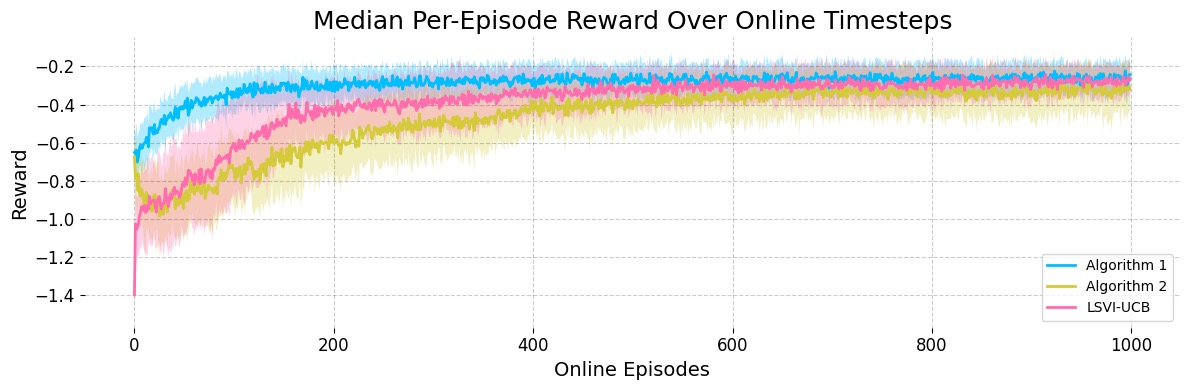
\includegraphics[width=0.8\linewidth]{figures/ch04/imgs/ac/reward.jpg}
    \caption[Per-episode reward of optimistic actor-critic methods on linear MDP Tetris]{Per-episode reward of Algorithms~\ref{alg:DOUHUA} and~\ref{alg:NORA} (labeled \texttt{Alg.\ 1} and \texttt{Alg.\ 2} in the legend), compared to a rare-switching version of LSVI-UCB \citep{jin2020provably} on a linear MDP Tetris task. Here, the condition required for Algorithm~\ref{alg:DOUHUA} holds, as we do not clip the $Q$-function estimates. Algorithm~\ref{alg:DOUHUA} outperforms LSVI-UCB, and Algorithm~\ref{alg:NORA} catches up after some time. Results are averaged over 30 trials.}
    \label{fig:median-reward}
\end{figure}

\begin{figure}[h]
    \centering
    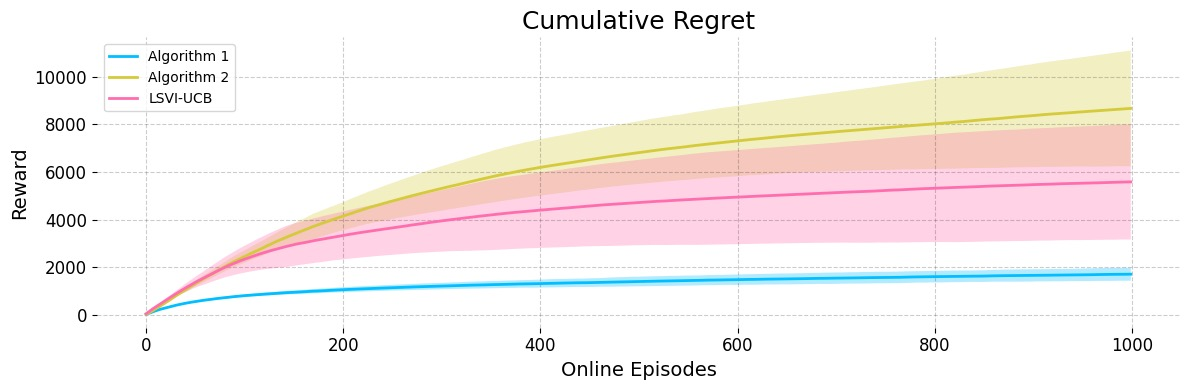
\includegraphics[width=0.8\linewidth]{figures/ch04/imgs/ac/regret.jpg}
    \caption[Cumulative regret of optimistic actor-critic methods on linear MDP Tetris]{Cumulative regret of Algorithms~\ref{alg:DOUHUA} and~\ref{alg:NORA} (labeled \texttt{Alg.\ 1} and \texttt{Alg.\ 2} in the legend) versus LSVI-UCB \citep{jin2020provably} on Tetris. This setting favors Algorithm~\ref{alg:DOUHUA}, which outperforms LSVI-UCB, while Algorithm~\ref{alg:NORA} also achieves $\sqrt{T}$ regret. Results are averaged over 30 trials.}
    \label{fig:cumulative-regret}
\end{figure}


\paragraph{Deep hybrid RL.} We compare practical deep RL variants of Algorithms~\ref{alg:NOAH-pi} and~\ref{alg:NOAH-star} (denoted Algorithms~1H and~2H, matching the plot labels in Figure~\ref{fig:average-return}) against Cal-QL \citep{nakamoto2023calql}. Algorithms~1H and~2H employ offline pretraining of both the actor and the critic, and the actor employs the soft actor-critic (SAC) update from \cite{haarnoja2018soft}. Additionally, Algorithm~2H omits the policy resets. Like Cal-QL, and unlike Algorithm~1H, Algorithm~2H takes a maximum over 10 randomly sampled actions from the policy to enhance exploration. This can be viewed as a computationally efficient version of optimism, or alternatively as approximately targeting $\pi^*$. 

Algorithm~2H outperforms Cal-QL, which in turn slightly outperforms Algorithm~1H. These results suggest that Algorithms~1H and~2H remain highly competitive, and may perform just as well as the state of the art in hybrid RL (Cal-QL) -- even without the use of pessimism. Our results support our theoretical findings that hybrid RL allows for computationally efficient actor-critic algorithms.


\begin{figure}[H]
    \centering
    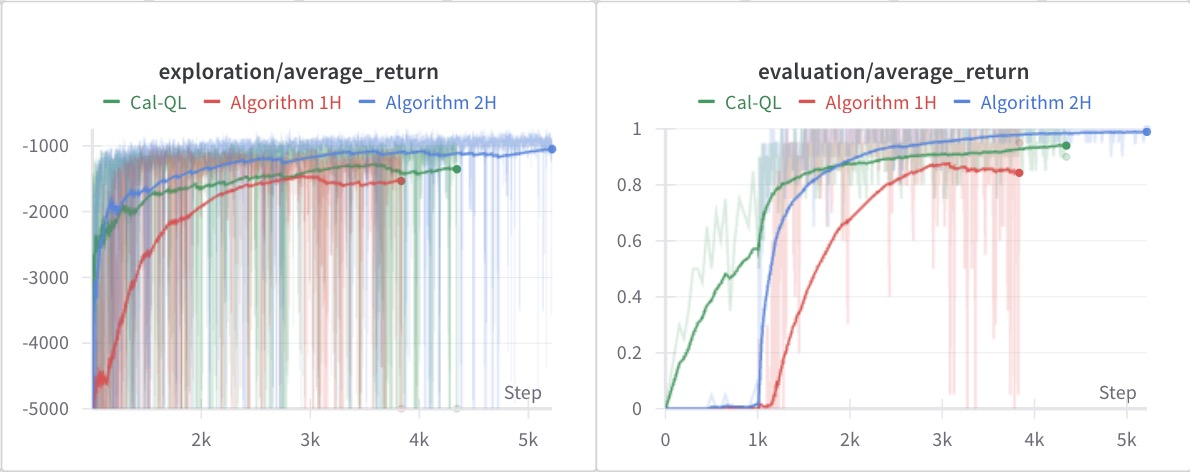
\includegraphics[width=0.8\linewidth]{figures/ch04/imgs/ac/hybrid.jpg}
    \caption[Deep hybrid RL return on AntMaze comparing non-optimistic actor-critics and Cal-QL]{Hybrid RL experiment on the \texttt{antmaze-medium-diverse-v2} task comparing Algorithms~1H and~2H (deep RL adaptations of Algorithms~\ref{alg:NOAH-pi} and~\ref{alg:NOAH-star}) against Cal-QL \citep{nakamoto2023calql} with offline pretraining. Algorithm~2H uses approximate optimism via action sampling and outperforms both Cal-QL and Algorithm~1H without pessimism. Evaluation plots show offline pretraining in the first 1000 steps, with exponential smoothing.}
    \label{fig:average-return}
\end{figure}

\section{Conclusions and future work}

To conclude, we resolve an open problem in the online RL literature by designing an actor-critic method, \aigen{Algorithm~\ref{alg:NORA}}, with general function approximation that achieves $1/\epsilon^2$ (and matching $\sqrt{T}$ regret) without making any reachability or coverage assumptions. This was achieved through several key ingredients in the algorithm design. By (1) performing optimistic exploration, (2) learning a critic off-policy without throwing away any data, (3) having the critic target $Q^*$ instead of $Q^{\pi^{(t)}}$ to ensure sufficient optimism and enable rare-switching critic updates, and (4) performing policy resets to control the deviation of the current policy from the greedy policy, we achieve the desired result in Theorem \ref{thm:nora-regret_bound}.

We resolve another open problem in the hybrid RL literature by providing a non-optimistic provably efficient actor-critic
algorithm that only additionally requires $N_{\off} \geq c_{\off}^*(\gF,\Pi)dH^4/\epsilon^2$ offline samples in exchange for omitting optimism. This, along with the result in Theorem \ref{thm:hybrid-nora-regret_bound}, shows that hybrid RL therefore allows for sample efficiency gains with optimistic algorithms and computational efficiency gains with non-optimistic algorithms. 

While Algorithm \ref{alg:NORA} is generally computationally inefficient, the insights gained are promising for empirical applications. 
Optimism is necessary for strategic exploration, and can be implemented via linear model bonuses \citet{agarwal2020pcpgpolicycoverdirected}, count-based exploration \citet{martin2017countbasedexplorationfeaturespace}, randomized value functions \citet{osband2019deepexplorationrandomizedvalue}, or random latent exploration \citet{mahankali2024randomlatentexplorationdeep}. An off-policy critic can be learned with the DDQN algorithm of \citet{vanhasselt2015deepreinforcementlearningdouble}, with the insight that one only needs to update when the TD error is high. Finally, an optimistic version of TD3 \citep{fujimoto2018addressing} with rare-switching critic updates and policy resets when necessary is a promising approach for a practical adaptation of Algorithm \ref{alg:NORA} in future work. Further numerical experiments and an extensive empirical study would constitute a very welcome contribution to the literature.

One may wish to incorporate bonus function classes as in \cite{agarwal2023vo, zhao2023nearlyoptimallowswitchingalgorithm}. With a rarely-updated bonus function class, updating the base critic every episode, one may be able to achieve sufficient optimism without targeting $Q^*$, but only if the sum of Q-functions is close to a scaled Q-function. 
Lastly, adapting the work of \citet{he2023nearly} to see if policy optimization can be minimax-optimal in linear MDPs, like \citet{wu2022nearlyoptimalpolicyoptimization} do for tabular MDPs, is a welcome contribution to the literature. 

% This is because updating the base function class every episode allows one to get past the moving target issue in targeting $Q^{\pi^{(t)}}$, while achieving sufficient optimism from the rare-switching bonuses. However, their techniques and analyses do not readily extend to general function approximation. Shrinking features does not necessarily shrink the Q-functions, for example. While reward-agnostic exploration is possible \citep{xie2022role}, it is unclear how to use this to avoid truncation, or employing rare-switching updates for bonuses, without involving an assumption on the structure of the bonuses. We suggest that the framework of \citet{zhao2023nearlyoptimallowswitchingalgorithm} provides a potential way forward, but leave this for future work. 

% Adapting the work of \citet{he2023nearly} to see if policy optimization can be (close to) minimax-optimal in linear MDPs is an appealing idea. However, in attempting to do so, we encountered a fundamental barrier. \citet{he2023nearly} require a monotonically decreasing Q-function estimate for technical reasons. This is not an issue when the target is $Q^*$ across all episodes, but becomes an issue when the target is $Q^{\pi^{(t)}}$, a moving target. When the policy is poor, and the Q-function is correctly estimated, enforcing the monotonicity constraint will render Q-function estimates for subsequent episodes wildly inaccurate. Resolving this technical issue would be a welcome contribution to the literature. 
